\batchmode
\documentclass[oneside,english]{book}
\usepackage{lmodern}
\usepackage[T1]{fontenc}
\usepackage[latin9]{inputenc}
\usepackage{geometry}
\geometry{verbose,tmargin=2.5cm,bmargin=2.5cm,lmargin=2.5cm,rmargin=2.5cm}
\setcounter{secnumdepth}{3}
\setcounter{tocdepth}{3}
\usepackage{color}
\usepackage{babel}
\usepackage{longtable}
\usepackage{float}
\usepackage{textcomp}
\usepackage{amsmath}
\usepackage{graphicx}
\newcommand{\uline}[1]{\underline{#1}}
\usepackage[unicode=true,
 bookmarks=false,
 breaklinks=false,pdfborder={0 0 1},backref=section,colorlinks=true]
 {hyperref}

\newcommand{\currentmonthyear}{%
  \ifcase\month
  \or January\or February\or March\or April\or May\or June%
  \or July\or August\or September\or October\or November\or December%
  \fi\space\number\year
}

\makeatletter

%%%%%%%%%%%%%%%%%%%%%%%%%%%%%% LyX specific LaTeX commands.
%% Because html converters don't know tabularnewline
\providecommand{\tabularnewline}{\\}

\makeatother

\begin{document}
\thispagestyle{empty}

\vspace*{3cm}

\begin{center}
\textbf{\huge{}{}The JETSPIN User Manual}{\huge{} }
\par\end{center}{\huge \par}

\bigskip{}

\begin{center}
{\large
M. Lauricella$^{1}$, G. Pontrelli$^{1}$, I. Coluzza$^{2}$,
D. Pisignano$^{3}$, S. Succi$^{4}$
}
\end{center}

\medskip{}

\begin{center}
{\large
$^{1}$Istituto per le Applicazioni del Calcolo ``Mauro Picone'',
Consiglio Nazionale delle Ricerche (CNR),\\
Via dei Taurini 19, 00185 Rome, Italy
}
\end{center}

\smallskip{}

\begin{center}
{\large
$^{2}$Center for Theoretical Biological Physics,
Rice University,\\
Houston, Texas, USA
}
\end{center}

\smallskip{}

\begin{center}
{\large
$^{3}$Department of Physics, University of Pisa,\\
Largo Bruno Pontecorvo 3, 56127 Pisa, Italy
}
\end{center}

\smallskip{}

\begin{center}
{\large
$^{4}$Center for Life Nano- \& Neuro-Science,
Istituto Italiano di Tecnologia (IIT),\\
Viale Regina Elena 291, 00161 Rome, Italy
}
\end{center}

\medskip{}

\begin{center}
\textbf{\large version 2.0-alpha - \currentmonthyear}
\end{center}

\newpage{}

\setcounter{page}{1}

\newpage{}

\vspace*{3cm}

\begin{center}
\textbf{\Large{}{}Disclaimer}{\Large{} }
\par\end{center}{\Large \par}

\bigskip{}

None of the authors, nor any contributor to the JETSPIN code or its
derivatives guarantee that the software and associated documentation
is free from error. Neither do they accept responsibility for any
loss or damage that results from its use. The responsibility for ensuring
that the software is fit for purpose lies entirely with the user.

\newpage{}

\vspace*{3cm}

\begin{center}
\textbf{\Large{}{}JETSPIN Acknowledgements}{\Large{} }
\par\end{center}{\Large \par}

\bigskip{}

\begin{center}
The software development process has received funding from the European
Research Council under the European Union's Seventh Framework Programme
(FP/2007-2013)/ERC Grant Agreement n. 306357 ``NANO-JETS''. 
\par\end{center}

\newpage{}

\vspace*{3cm}

\begin{center}
\textbf{\Large{}{}About JETSPIN}{\Large{} }
\par\end{center}{\Large \par}

\bigskip{}

The code is licensed under Open Software License v. 3.0 (OSL-3.0).
The full text of the licence can be found on the website: http://opensource.org/licenses/OSL-3.0

If results obtained with this code are published, an appropriate citation
would be:

Marco Lauricella, Giuseppe Pontrelli, Ivan Coluzza, Dario Pisignano,
Sauro Succi, JETSPIN: A specific-purpose open-source software for
electrospinning simulations of nanofibers, \textit{Computer Physics
Communications}, 197 (2015), 227-238.

\newpage{} \tableofcontents{}

\newpage{}

\chapter{Introduction\label{chap:Introduction}}

\section*{Scope of Chapter}

This chapter describes the design and directory structure of JETSPIN.

% JETSPIN Package documentation

\section{The JETSPIN Package\label{sec:The-JETSPIN-Package}}

In the recent years, electrospun nanofibers have gained a considerable
industrial interest due to many possible applications, such as tissue
engineering, air and water filtration, drug delivery and regenerative
medicine. In particular, the high surface-area ratio of the fibers
offers an intriguing prospect for technological applications. As consequence,
several studies were focused on the characterization and production
of uni-dimensionally elongated nanostructures. A number of reviews
\cite{li2004electrospinning,greiner2007electrospinning,carroll2008nanofibers,huang2003review,persano2013industrial}
and books \cite{yarin2014fundamentals,wendorff2012electrospinning,pisignanoelectrospinning}
concerning electrospinning have been published in the last decade.

Typically, electrospun nanofibers are produced at laboratory scale
by the uniaxial stretching of a jet, which is ejected at the nozzle
from a charged polymer solution. The initial elongation of a jet can
be produced by applying an externally electrostatic field between
the spinneret and a conductive collector. Electrospinning involves
mainly two sequential stages in the uniaxial elongation of the extruded
polymer jet: an initial quasi steady stage, in which the electric
field stretches the jet in a straight path away from the nozzle of
the ejecting apparatus, and a second stage characterized by a bending
instability induced from small perturbations, which misalign the jet
from its axis of elongation \cite{zeng2006numerical}. These small
disturbances may originate from mechanical vibrations at the nozzle
or from hydrodynamic-aerodynamic perturbations within the experimental
apparatus. Such a misalignment provides an electrostatic-driven bending
instability before the jet reaches the conductive collector, where
the fibers are finally deposited. As a consequence, the jet path length
between the nozzle and the collector increases, and the stream cross-section
undergoes a further decrease. The ultimate goal of electrospinning
process is to minimize the radius of the collected fibers. By a simple
argument of mass conservation, this is tantamount to maximizing the
jet length by the time it reaches the collecting plane. By the same
argument, it is therefore of interest to minimize the length of the
initial stable jet region. Consequently, the bending instability is
a desirable effect, as it produces a higher surface-area-to-volume
ratio of the jet, which is transferred to the resulting nanofibers
\cite{feng2003stretching}.

Computational models provide a useful tool to elucidate the physical
phenomenon and provide information which might be used for the design
of electrospinning experiments. Numerical simulations can be used
to improve the capability of predicting the key processing parameters
and exert a better control on the resulting nanofiber structure. In
recent years, with a renewed interest in nanotechnology, electrospinning
studies attracted the attention of many resarchers both from modeling,
computational and experimental point of view \cite{reneker2000bending,yarin2001taylor,fridrikh2003controlling,theron2004experimental,lu2006computer,zeng2006numerical}.
Although some author uses dissipative particle dynamics (DPD) mesoscale
simulation method into electrospinning study \cite{wang2013simulation},
most models usually treat the jet filament as a series of discrete
elements ({\em beads}) obeying the equations of continuum mechanics
\cite{reneker2000bending,yarin2001taylor}. Each bead is subject to
different types of interactions, such as long-range Coulomb repulsion,
viscoelastic drag, the external electric field. The main aim of such
models is to explain the complexity of the resulting dynamics and
provide the set of parameters driving the optimal process. The effect
of fast-oscillating loads on the bending instability have been explored
in an extensive modeling and computational study \cite{coluzza2014ultrathin}.

JETSPIN delivers a FORTRAN code especially designed to simulate the
electrospinning process in a variety of different conditions and experimental
settings. This comprehensive platform is devised such that different
cases and input variables can be described and simulated. The framework
is developed to exploit several computational architectures, both
serial and parallel.

JETSPIN, as open-source software, can be used to carry out a systematic
sensitivity analysis over a broad range of parameter values. The results
of simulations provide valuable insight on the physics of the process
and can be used to assess experimental procedures for an optimal design
of the equipment and to control processing strategies of technological
advanced nanofibers.

\textbf{The JETSPIN code is freely downloadable at the web site: }

\bigskip{}

\begin{center}
\href{http://www.nanojets.eu}{http://www.nanojets.eu}
\par\end{center}


% JETSPIN structure documentation

\section{Structure\label{sec:Structure}}

JETSPIN is written in free format FORTRAN90, and it consists of approximately
160 subroutines. The source exploits the modular approach provided
by the programming language. All the variables having in common description
of certain features or method are grouped in modules. The convention
of explicit type declaration is adopted, and all the arguments passed
in calling sequences of functions or subroutines have defined intent.
We use the PRIVATE and PUBLIC accessibility attributes in order to
decrease error-proneness in programming.

The main routines have been gathered in the \texttt{main.f90} file,
which drives all the CPU-intensive computations needed for the capabilities
mentioned below. The variables describing the main features of nanofibers
(position, velocity, etc.) are declared in the \texttt{nanojet\_mod.f90}
file, which also contains the main subroutines for the memory management
of the fundamental data of the simulated system. Since the size system
is strictly time-dependent, JETSPIN exploits the dynamic array allocation
features of FORTRAN90 to assign the necessary array dimensions. In
particular, the size system is modified by the routines \texttt{add\_jetbead}
and \texttt{erase\_jetbead}, while the decision of the main array
size, declared as \texttt{mxnpjet}, is handled by the routine \texttt{reallocate\_jet}.
The sizes of various service bookkeeping arrays are handled within
a parallel implementation strategy, witch exploits few dedicated subroutines
(see Sec \ref{sec:Parallelization}). All the implemented time integrators
are written in the \texttt{integrator\_mod.f90} file, which contains
the routine \texttt{driver\_integrator} to select the proper integrator,
as indicated in the input file. All the terms of equations of motion
for the implemented model (see Sec \ref{sec:Equation-of-Motion})
are computed by routines located in the \texttt{eom\_mod.f90} file,
which call other subroutines in the files \texttt{coulomb\_force\_mod.f90},
\texttt{viscoelastic\_force\_mod.f90} and \texttt{support\_functions\_mod.f90}.
A summarizing scheme of the main JETSPIN program in the \texttt{main.f90}
file has been sketched in Fig \ref{Fig:Structure-program}.

The user can carry out simulations of nanofibers without a detailed
understanding of the structure of JETSPIN code. All the parameters
governing the system can be defined in the input file (see Sec \ref{sec:Input-file}),
which is read by routines located in the \texttt{io\_mod.f90} and
\texttt{parse\_mod.f90} files. Instead, the user should be acquainted
with the model described in Cap \ref{chap:JETSPIN-Model-and}. The
content of the output file is completely customizable by the input
file as described in Sec \ref{sec:Input-file}, and it can report
different time-averaged observables computed by routines of the module
\texttt{statistic\_mod} (see Sec \ref{sec:Output-files}). The routines
in the \texttt{error\_mod.f90} file can display various warning or
error banners on computer terminal, so that the user can easily correct
the most common mistakes in the input file.

JETSPIN is supplied as a single UNIX compressed (tarred and gzipped)
directory with four sub-directories. All the source code files are
contained in the \textit{source} sub-directory. The \textit{examples}
sub-directory contains different test cases that can help the user
to edit new input files. The \textit{build} sub-directory stores a
UNIX \texttt{makefile} that assembles the executable versions of the
code both in serial and parallel versions with different compilers.
It is invoked from the repository root while using the \textit{source}
sub-directory as its working directory (see Section
\ref{sec:Compiling-the-Source}); it does not need to be copied.
Finally, after JETSPIN was compiled, the \textit{execute} sub-directory
contains the binary executable file, where it can be run.

\begin{figure}
\begin{centering}
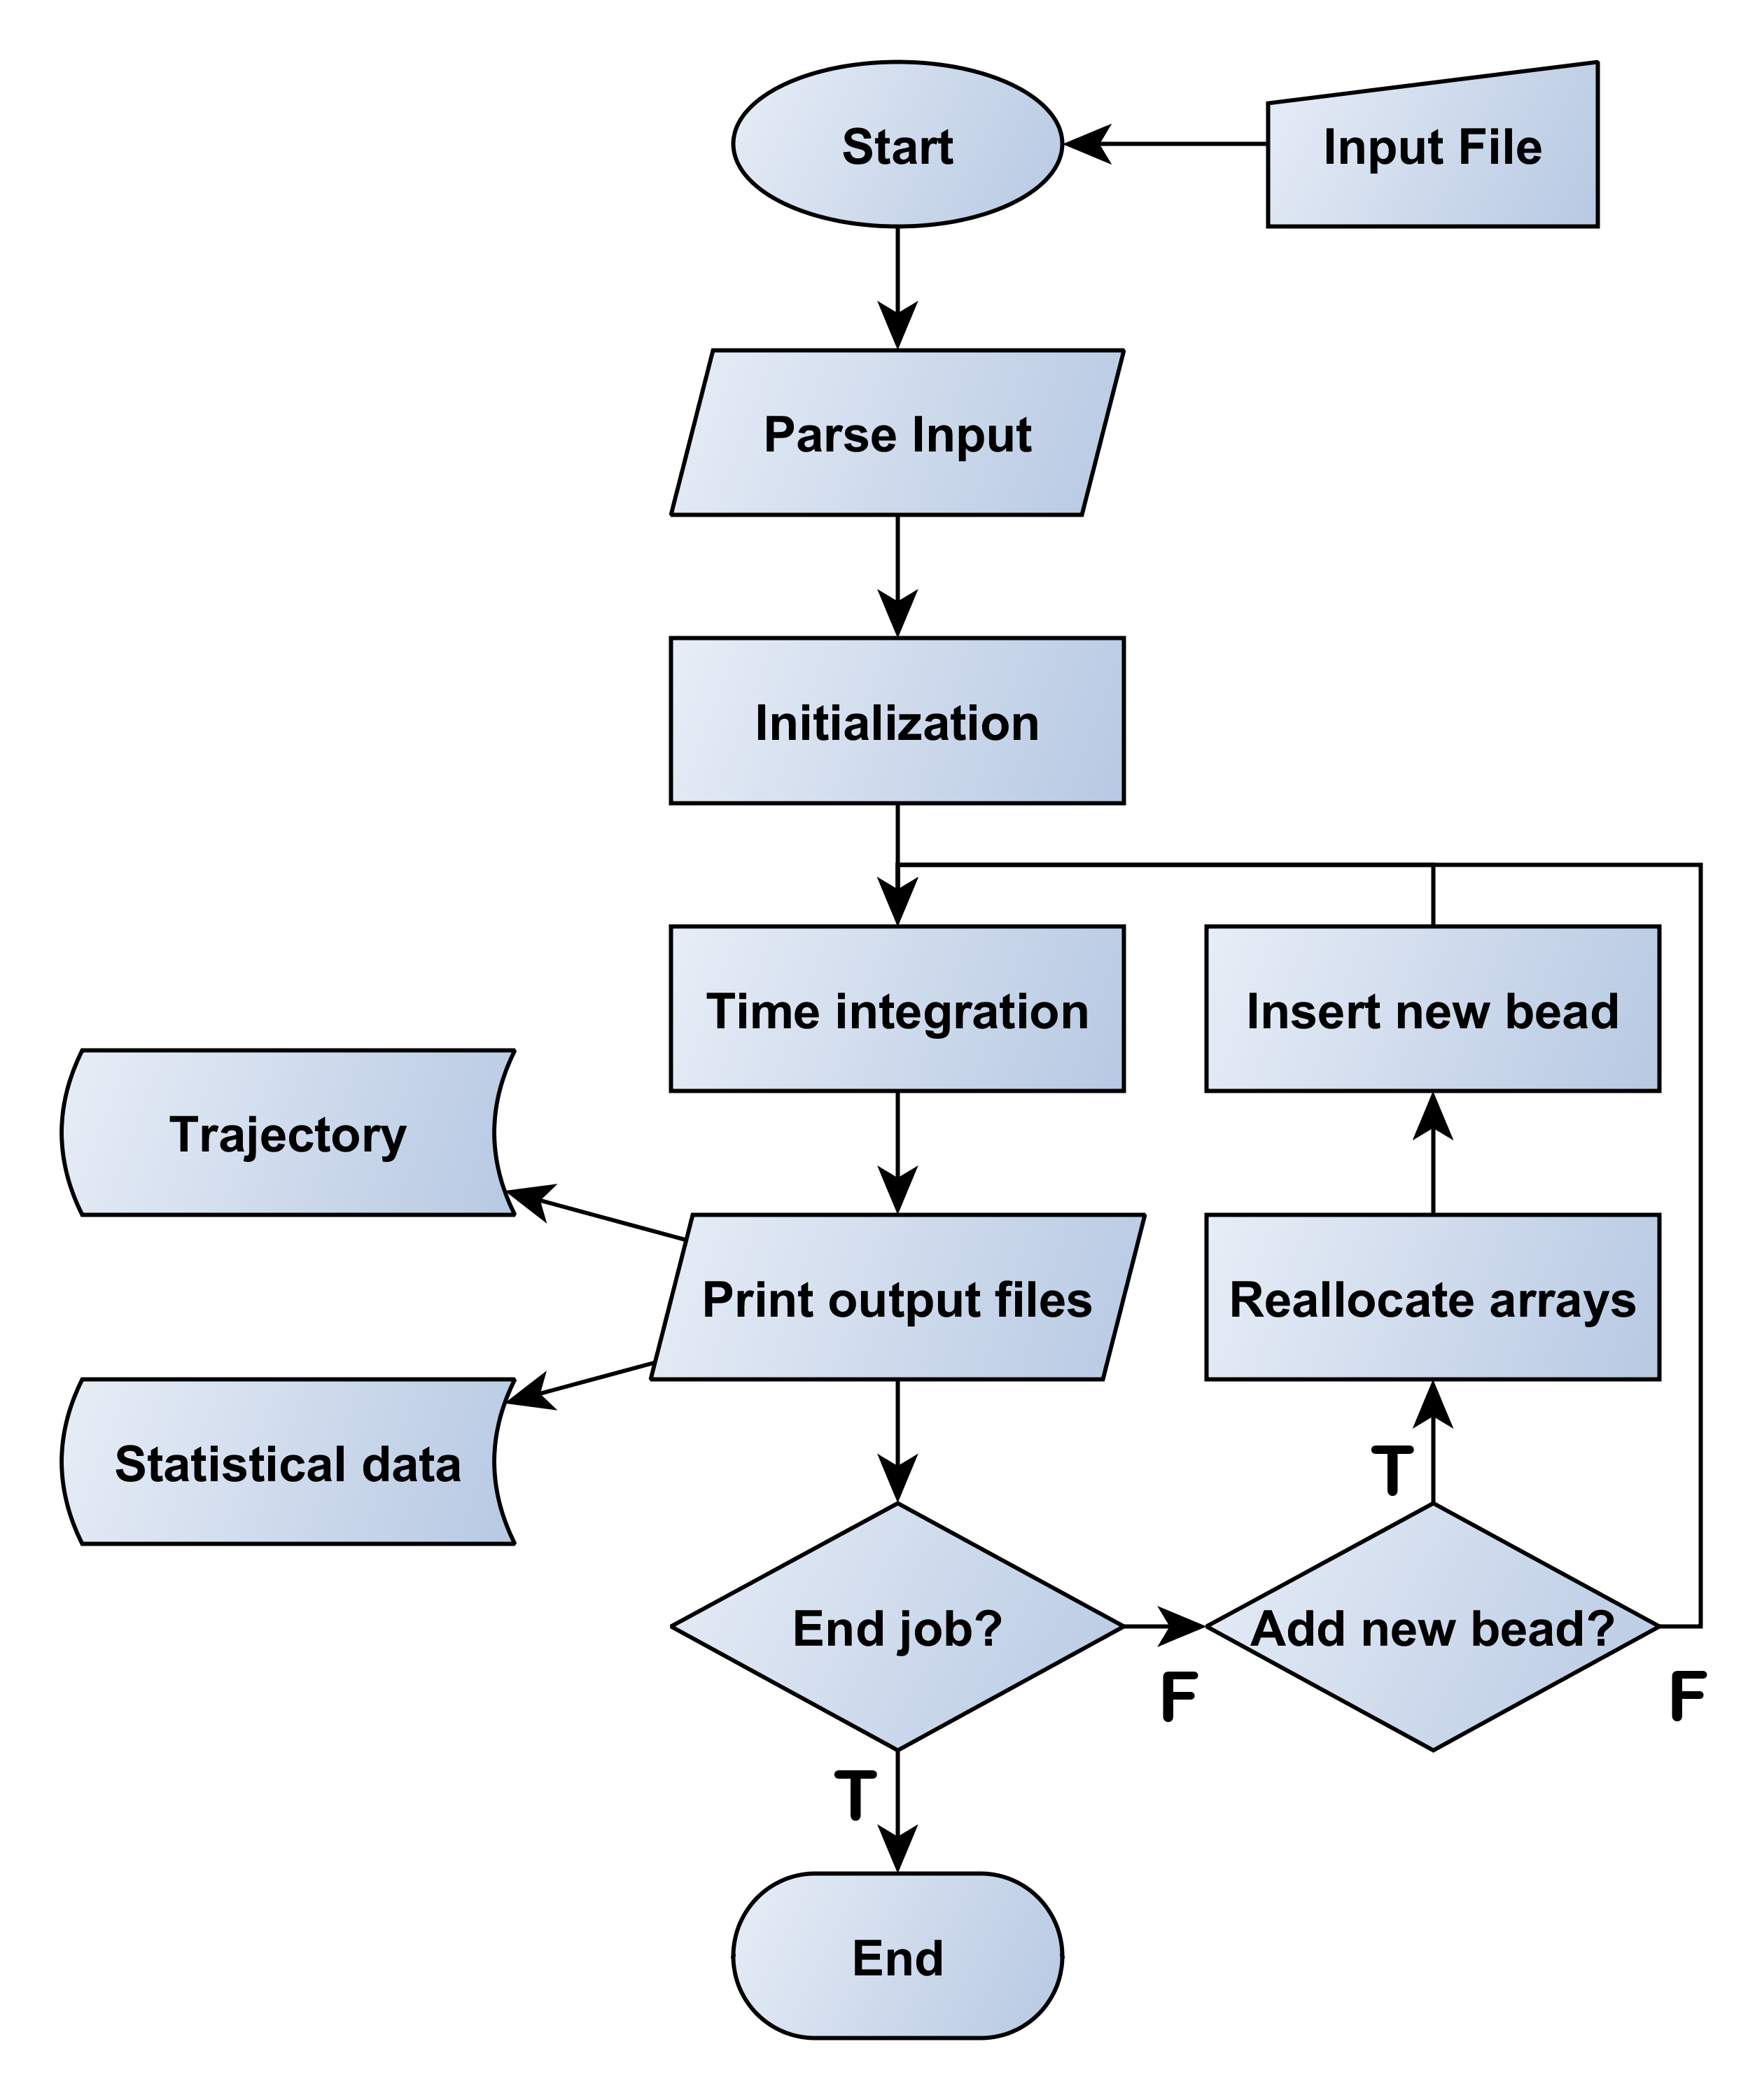
\includegraphics[scale=0.18]{figure01}
\par\end{centering}
\protect\caption{Structure of the main JETSPIN program.}

\label{Fig:Structure-program}
\end{figure}


% JETSPIN parallelization documentation

\section{Parallelization\label{sec:Parallelization}}

The parallel infrastructure of JETSPIN incorporates the necessary
data distribution and communication structures. The parallel strategy
underlying JETSPIN is the Replicated Data (RD) scheme\cite{smith1991molecular},
where fundamental data of the simulated system are reproduced on all
processing nodes. In simulations of nanofibers, the fundamental data
consist of position, velocity, and viscoelastic stress arrays of each
bead in which the nanojet is discretised (see below Cap \ref{chap:JETSPIN-Model-and}).
Further data defining mass and charge of each bead are also replicated.
However, all auxiliary data are distributed in equal portion of data
(as much as possible) for each processor. Despite being available
other parallel strategies such as the Domain Decomposition\cite{brown1993domain},
our experience has shown that such volume of data is by no means prohibitive
on current parallel computers.

By the RD scheme, we adopt in JETSPIN a simple communication strategy
of the communication between nodes, which is handled by global summation
routines. The module \texttt{version\_mod} located in the \texttt{parallel\_version\_mod.f90}
file contains all the global communication routines which exploit
the MPI (Message Passing Interface) library. Note that a FORTRAN90
compiler and an MPI implementation for the specific machine architecture
are required in order to compile JETSPIN in parallel mode. An alternative
version of the module \texttt{version\_mod} is located in the \texttt{serial\_version\_mod.f90}
file, and it can be easily selected by appropriate flags in the \texttt{makefile}
at compile time. By selecting this version, JETSPIN can also be run
on serial computers without modification, even though the code has
been designed to run on parallel computers.

The size system is strictly time-dependent as mentioned in Sec \ref{sec:Structure}
and, therefore, the memory of various service bookkeeping arrays is
dynamically distributed over all the processing nodes. In particular,
the bookkeeping array size, declared as \texttt{mxchunk}, is managed
by the routine \texttt{set\_mxchunk}. All the beads of the discretised
nanofiber are assigned at every time step to a specific node by the
routine \texttt{set\_chunk}, and their temporary data are stored in
bookkeeping arrays belonging to the assigned node. It is worth stressing
that the communication latency makes the parallelization efficiency
strictly dependent on the system size. Therefore, we only advice the
use of JETSPIN in parallel mode whenever the user expects a system
size with at least 50 beads for each node (further details in Ref
\cite{lauricella2015jetspin}).


% JETSPIN compiling documentation

\section{Compiling the Source Code\label{sec:Compiling-the-Source}}

The \textit{build} sub-directory stores a UNIX \textbf{Makefile} that
assembles serial and parallel executable versions with different
compilers. JETSPIN may be compiled on any UNIX platform. From the root
of the repository, invoke this file directly while making \textit{source}
the working directory; there is no need to copy the Makefile. Use

\bigskip{}

\texttt{make -C source -f ../build/Makefile target}

\bigskip{}

where \texttt{target} is one of the options reported in
Table~\ref{Tab:targets}. Object and module files are generated in
\textit{source}, and the resulting \texttt{main.x} executable is placed
in \textit{execute}. For example, the serial GFortran build is produced
with

\bigskip{}

\texttt{make -C source -f ../build/Makefile gfortran}

\bigskip{}

and the corresponding Open MPI build with target
\texttt{gfortran-mpi}. Build products can be removed with target
\texttt{clean} using the same command form.

NVIDIA HPC SDK provides separate CPU-only and OpenACC build targets. On a
module-based installation, first load the SDK and verify that its MPI wrapper
uses NVFORTRAN:

\begin{verbatim}
module purge
module use /opt/nvidia/hpc_sdk/modulefiles
module load nvhpc/24.3
nvfortran --version
mpif90 --showme:command
\end{verbatim}

The serial and MPI CPU-only builds are selected respectively with
\texttt{nvfortran} and \texttt{nvfortran-mpi}. The latter requires
\texttt{mpif90 --showme:command} to report \texttt{nvfortran}.
Neither target enables OpenACC offloading.

The \texttt{nvfortran-openacc} target enables single-GPU OpenACC
offloading. Its default values target compute capability 8.0, including
NVIDIA A30 and A100 GPUs, and the CUDA 12.3 toolkit distributed with HPC SDK
24.3. It also selects the \texttt{nofma} GPU option to preserve the numerical
behaviour of the nearly straight three-point curvature calculation:

\begin{verbatim}
make -C source -f ../build/Makefile nvfortran-openacc
\end{verbatim}

The OpenACC GPU and host-validation targets expose the standard
\texttt{\_OPENACC} preprocessing macro.
Accelerator imports, initialization, Coulomb dispatch, and equation-of-motion
dispatch are enclosed by this macro. CPU targets preprocess the same sources
without defining it, so accelerator calls are absent from their compiled
translation units rather than being retained as no-op runtime branches.

Another device architecture or installed CUDA toolkit can be selected through
the \texttt{GPUCC} and \texttt{CUDA\_VERSION} Make variables. The
compute capability is passed without the \texttt{cc} prefix; for example:

\begin{verbatim}
make -C source -f ../build/Makefile nvfortran-openacc \
  GPUCC=90 CUDA_VERSION=12.3
\end{verbatim}

Target \texttt{nvfortran-openacc-host} compiles the OpenACC control path
for host execution. It is intended for compiler and numerical validation when
an NVIDIA device is unavailable and is not a GPU performance build. Before a
device run, \texttt{nvidia-smi} and \texttt{nvaccelinfo} should both
confirm that the selected GPU is visible.

Target \texttt{nvfortran-openacc-host-forces} is a development-only GPU build
that evaluates the evaporative Coulomb and Maxwell geometric forces with the
trusted host routines and copies their results back to the device. It is useful
for numerical isolation, but the per-stage transfers make it unsuitable for
performance measurements or production simulations.

On Windows system we advice the user to compile JETSPIN under the
command-line interface Cygwin \cite{racine2000cygwin}. Finally, the
binary executable file can be run in the \textit{execute} sub-directory.
Note that a FORTRAN 90 compiler is necessary in order to compile JETSPIN.
Further, a Message Passing Interface Implementation should be also
present, if the user wishes to compile JETSPIN in parallel mode. We
recommend GFORTRAN as FORTRAN 90 compiler, but IFORT-Intel(R) Fortran
Compiler or G95 can also be used. As Message Passing Interface Implementation,
we suggest to use that provided by the Open MPI Project.

\begin{table}[H]
\begin{centering}
\begin{tabular}{p{0.29\textwidth}p{0.65\textwidth}}
\hline
\textbf{target:}  & \textbf{meaning:}\tabularnewline
\hline
\hline
gfortran  & compile in serial mode using the GFortran compiler.\tabularnewline
gfortran-mpi  & compile in parallel mode using the GFortran compiler and the Open
Mpi library.\tabularnewline
cygwin  & compile in serial mode using the GFortran compiler under the command-line\tabularnewline
 & interface Cygwin for Windows.\tabularnewline
cygwin-mpi  & compile in parallel mode using the GFortran compiler and the Open
Mpi library\tabularnewline
 & under the command-line interface Cygwin for Windows (note a precompiled\tabularnewline
 & package of the Open Mpi library is already available on Cygwin).\tabularnewline
intel  & compile in serial mode using the Intel compiler.\tabularnewline
intel-mpi  & compile in parallel mode using the Intel compiler and the Intel Mpi
library.\tabularnewline
intel-openmpi  & compile in parallel mode using the Intel compiler and the Open Mpi
library.\tabularnewline
nvfortran & compile in serial CPU mode using NVIDIA Fortran; OpenACC offloading
is disabled.\tabularnewline
nvfortran-mpi & compile in parallel CPU mode using an MPI wrapper configured
with NVIDIA Fortran; OpenACC offloading is disabled.\tabularnewline
nvfortran-openacc & compile a single-GPU OpenACC executable; configure the
device with \texttt{GPUCC} and \texttt{CUDA\_VERSION}.\tabularnewline
nvfortran-openacc-host & compile the OpenACC code path for host-only validation.\tabularnewline
nvfortran-openacc-host-forces & compile the GPU path with development-only
host force evaluation and per-stage transfers.\tabularnewline
help  & return the list of possible target choices\tabularnewline
\hline
\end{tabular}
\par\end{centering}
\protect\caption{List of targets for several common workstations and parallel computers,
which can be used with the Makefile in the \textit{build} sub-directory.}

\label{Tab:targets}
\end{table}


% JETSPIN running documentation

\section{Running JETSPIN\label{sec:Running-JETSPIN}}

In order to run the JETSPIN executable (main.x) the user should prepare
the input file following the hints provided in Section \ref{sec:Input-file}.
The test cases located in \textit{examples} sub-directory can be used
as starting point for editing the input file. As JETSPIN is executed,
the program will look for the input file, named \texttt{input.dat},
in the same directory, where the executable was called. For instance,
if JETSPIN is called in the \textit{execute} sub-directory, the code
will look for the file \texttt{input.dat}, which must have been put
in the same sub-directory.

The JETSPIN code can be executed in serial mode by the command\texttt{ }

\bigskip{}

\texttt{./main.x}

\bigskip{}

or in parallel mode by the command

\bigskip{}

\texttt{mpirun -np \$ncpu ./main.x}

\bigskip{}
 where \texttt{\$ncpu} is the number of CPUs used in parallel (e.g.
\texttt{mpirun -np 4 ./main.x} in order to run JETSPIN in parallel
mode on 4 CPUs).

A successful run of JETSPIN will generate several output files, which
appear in the directory, where the executable was called. The output
files will be produced only if their writing was explicitly requested
in input file by using proper directives (see Section \ref{sec:Input-file}).
A detailed description of the generated output files is provided in
Section \ref{sec:Output-files}. Briefly, the main output files are
the files \texttt{statdat.dat},\texttt{ traj.xyz} and \texttt{frame\%06d.xyz},
which are human readable. The contains a catalogue of instantaneous
or blocked averaged values of several variables, which can be used
for temporal or statistical analysis in post-processing. The \texttt{traj.xyz}
file provides a time ordered sequence of configurations to facilitate
further analysis of the jet dynamics, while the \texttt{frame\%06d.xyz}
file, reports the same information in splitted files, one for each
registered time frame. Further, as JETSPIN is running, a series of
lines will be printed in the terminal window, providing several information
as requested by suitable directives in input file (see Section \ref{sec:Input-file}).
Also present will be the \texttt{save.dat} file, which contains the
accumulated data for computing statistical quantities and other quantities
defining the current simulation. This file is intended to be used
together with the input file for restarting a JETSPIN job (see Section
\ref{sec:Restarting-JETSPIN}), and it is \textit{not} human readable.


% JETSPIN restarting documentation

\section{Restarting JETSPIN\label{sec:Restarting-JETSPIN}}

A simulation can be restarted after normal termination or error termination,
if the last was due to inadequate time allocation. In order to restart
a JETSPIN job the file \texttt{input.dat} is again required together
with the file \texttt{restart.dat}, which is the exact copy of the
\texttt{save.dat} file created by the previous job. In particular,
the \texttt{save.dat} file was written by JETSPIN at regular time
interval during the previous simulation. The file \texttt{save.dat}
is \textit{not} human readable, and it should be renamed as \texttt{restart.dat},
and located in the same directory of input file. If the user attempts
to restart JETSPIN without the \texttt{restart.dat} file, the job
will immediately exit with error. Note that the directive ``\textit{restart
yes}'' needs to be added in input file in order to restart a previous
JETSPIN job (see Section \ref{sec:Input-file}). Further, whenever
a job is restarted, it is also possible to reset the accumulated statistical
data, collected in the previous run, by adding the directive ``\textit{restart
reset}'' in input file. It is worth stressing that JETSPIN will append
new data to the files \texttt{statdat.dat},\texttt{ traj.xyz} , while
all the other output files will be \textbf{overwritten} (included
the \texttt{save.dat} file). Thus, the user is advised to keep backup
copies of the \texttt{restart.dat} file, noting the times it was written,
to help you avoid going right back to the start of a simulation.

The same restarting procedure can be also used for extending a simulation
beyond its initial allocation of timesteps. In this case, the directive
\textit{timesteps} should be adjusted in input file to the new total
number of steps required for the simulation. For instance, if a 10000
step simulation needs to be extended by a further 5000 steps, the
user should use the directive ``\textit{timesteps 15000}'' in the
input file and include the ``\textit{restart yes}'' directive. Further,
the restarting procedure can be useful in the event of machine failure.
Here, the job can be restarted in the same way from the \texttt{save.dat}
file, which is written at regular time intervals in order to meet
just such an emergency. We stress that the procedure is not foolproof
in the last event, since the job could be crash while the \texttt{save.dat}
file is being written.


\newpage{}

\chapter{JETSPIN Model and Algorithms\label{chap:JETSPIN-Model-and}}

\section*{Scope of Chapter}

This chapter describes the model and simulation algorithms incorporated
into JETSPIN.

% JETSPIN EoM documentation

\section{Equations of Motion\label{sec:Equation-of-Motion}}

The model implemented in JETSPIN is an extension of the Lagrangian
discrete model introduced by Reneker et al. \cite{reneker2000bending}
(in the following text referred as Ren model). The model provides
a compromise of efficiency and accuracy by representing the filament
as a series of $n$ beads (jet beads) at mutual distance $l$ connected
by viscoelastic elements. The length $l$ is typically larger than
the cross-sectional radius of the filament, but smaller than the characteristic
lengths of other observables of interest (e.g. curvature radius).
Each $i-th$ bead has mass $m_{i}$ and charge $q_{i}$ (not necessarily
equal for all the beads). The nanofiber is modeled as a viscoelastic
fluid following the approach developed in Ref. \cite{pontrelli2014electrospinning},
and the stress $\sigma_{i}$ for the element connecting bead $i$
with bead $i+1$ is given by the viscoelastic constitutive equation:

\begin{equation}
\frac{d\sigma_{i}}{dt}=-\frac{1}{t_{0}}\left(\sigma_{i}-\sigma_{HB}\right),\label{eq:huang-garcia}
\end{equation}
where $t_{0}$ is the relaxation time and $\sigma_{HB}$ is the Herschel\textendash Bulkley
stress. Note that the relaxation time is give as

\begin{equation}
t_{0}=\frac{\mu}{G},\label{eq:relaxation-time}
\end{equation}
where $G$ is the elastic modulus and $\mu$ the viscosity of the
fluid jet, while $\sigma_{HB}$ reads

\begin{equation}
\sigma_{HB}=\sigma_{Y}+K_{\upsilon e}\left(\frac{1}{l_{i}}\frac{dl_{i}}{dt}\right)^{n_{\upsilon e}}.\label{eq:Herschel=00003D002013Bulkley}
\end{equation}
In the previous expression, $K_{\upsilon e}$ is the flow consistency
index with dimensions $\text{g}\text{s}^{ne-2}\text{cm}^{-1}$, $\sigma_{Y}$
the yield stress, $n_{\upsilon e}$ the flow behavior index, $t$
the time, and $l_{i}$ the length of the element connecting bead $i$
with bead $i+1$. Note that it is possible to define an effective
viscosity $\mu_{eff}$ as

\begin{equation}
\mu_{eff}=K_{\upsilon e}\left(\frac{1}{l_{i}}\frac{dl_{i}}{dt}\right)^{n_{\upsilon e}-1}.\label{eq:effective-viscosity}
\end{equation}
It is worth stressing that the case $K_{\upsilon e}=\mu$, $n_{\upsilon e}=1$
and $\sigma_{Y}=0$ recovers the Maxwellian fluid model. Keeping the
last case in mind, for convenience sake, we write

\begin{equation}
K_{\upsilon e}=k_{\upsilon e}\mu,\label{eq:rescaled-prefactor}
\end{equation}
with $k_{\upsilon e}$ the flow consistency index re-scaled by $\mu$,
and the viscoelastic constitutive equation is rearranged as

\begin{equation}
\frac{d\sigma_{i}}{dt}=-\frac{G}{\mu}\left[\sigma_{i}-\sigma_{Y}+k_{\upsilon e}\mu\left(\frac{1}{l_{i}}\frac{dl_{i}}{dt}\right)^{n_{\upsilon e}}\right],\label{eq:stress-ode}
\end{equation}
The last constitutive equation allows the modeling of several fluids
as, for example, Bingham fluids ( $\sigma_{Y}>0$ ), shear-thinning
fluids ( $n_{\upsilon e}>1$ ), shear-thickening fluid ( $n_{\upsilon e}<1$
) .

As alternative, it is possible to activate the Kelvin\textendash Voigt
model \cite{barnes1989introduction} (see Tab \ref{tab:inputlist}).
In the last case, Eq \ref{eq:stress-ode} is replaced by

\begin{equation}
\frac{d\sigma_{i}}{dt}=G\frac{1}{l_{i}}\frac{dl_{i}}{dt}+\mu\frac{1}{l_{i}}\frac{d\upsilon_{i}}{dt}.\label{eq:stress-ode-KV}
\end{equation}

Given $a_{i}$ the cross-sectional radius of the filament at the bead
$i$, the viscoelastic force $\vec{\textbf{f}}_{\upsilon e}$ pulling
bead $i$ back to $i-1$ and towards $i+1$ is

\begin{equation}
\vec{\textbf{f}}_{\upsilon e,i}=-\pi a_{i}^{2}\sigma_{i}\cdot\vec{\textbf{t}}_{i}+\pi a_{i+1}^{2}\sigma_{i+1}\cdot\vec{\textbf{t}}_{i+1}\text{,}
\end{equation}
where $\vec{\textbf{t}}_{i}$ is the unit vector pointing bead $i$
from bead $i-1$. The surface tension force $\vec{\textbf{f}}_{st}$
for the $i-th$ bead is given by

\begin{equation}
\vec{\textbf{f}}_{st,i}=k_{i}\cdot\pi\left(\frac{a_{i}+a_{i-1}}{2}\right)^{2}\alpha\cdot\vec{\textbf{c}}_{i}\text{,}
\end{equation}
where $\alpha$ is the surface tension coefficient, $k_{i}$ is the
local curvature, and $\vec{\textbf{c}}_{i}$ is the unit vector pointing
the center of the local curvature from bead $i$. Note the force $\vec{\textbf{f}}_{st}$
is acting to restore the rectilinear shape of the bending part of
the jet.

In the electrospinning experimental configuration an intense external
electric potential $\Phi_{0}$ is applied between the spinneret and
a conducting collector located at distance $h$ from the injection
point. As consequence, each $i-th$ bead endures the electric force

\begin{equation}
\vec{\textbf{f}}_{el,i}=e_{i}\frac{\Phi_{0}}{h}\cdot\vec{\textbf{x}}\text{,}
\end{equation}
where $\vec{\textbf{x}}$ is the unit vector pointing the collector
from the spinneret and assumed along the $x$ axis. Note that in Ren
model the electric field $\Phi_{0}$ is assumed to be static in order
to avoid the computationally expensive integration of Poisson equation,
whereas in reality $\Phi$ is depending on the net charge of the nanofiber
so as to maintain constant the potential at the electrodes. The latter
issue was elegantly addressed by Kowalewski et al. \cite{kowalewski2009modeling},
and its implementation in JETSPIN will be planned. Further, it is
possible to impose a time dependent external electric potential described
by a rectangular waveform with amplitude $\Phi_{0}$ and frequency
given in input file (see Section \ref{sec:Input-file}).

The net Coulomb force $\vec{\textbf{f}}_{c}$ acting on the $i-th$
bead from all the other beads is given by

\begin{equation}
\vec{\textbf{f}}_{c,i}=\sum_{\substack{j=1\\
j\neq i
}
}^{n}\frac{q_{i}q_{j}}{R_{ij}^{2}+a_{j}^{2}}\cdot\vec{\textbf{u}}_{ij}\text{,}
\end{equation}
where $R_{ij}=\left[\left(x_{i}-x_{j}\right)^{2}+\left(y_{i}-y_{j}\right)^{2}+\left(z_{i}-z_{j}\right)^{2}\right]^{1/2}$,
and $\vec{\textbf{u}}_{ij}$ is the unit vector pointing the $i-th$
bead from $j-th$ bead. Note that $j-th$ charge is assumed to induces
a field from its outer shell of the fiber (a charged ring of radius
$a_{j}$) and not from the center line (the particle-like point) as
implemented in the original Ren model. Although the Ren model provides
a reasonable description for the spiral motion of the jet, the last
term $\vec{\textbf{f}}_{c}$ introduces mathematical inconsistencies
due to the discretization of the fiber into point-charges. Different
approaches were developed to overcome this issue which usually imply
strong approximations\cite{feng2002stretching,feng2003stretching,hohman2001electrospinning}.
Other strategies use a less crude approximation by accounting for
the actual electrostatic form factors between two interacting sections
of a charged fiber\cite{kowalewski2005experiments} or involving more
sophisticated methods which exploit the tree-code hierarchical force
calculation algorithm\cite{kowalewski2009modeling}. In JETSPIN it
is possible to activate the dynamic refinement algorithm to recover
a finer discretization of the jet (see Sec \ref{sec:Dynamic-refinement}).

Although usually much smaller than the other driving forces, the body
force due to the gravity is computed in the model by the usual expression

\begin{equation}
\vec{\textbf{f}}_{g,i}=m_{i}g\cdot\vec{\textbf{x}},
\end{equation}
where $g$ is the gravitational acceleration.

As shown in experimental evidences \cite{spinning1991science}, the
air drag force affects the dynamics of the nanofiber. The extended
stochastic model developed in Refs \cite{lauricella2016refinement,Lauricella2015dissipative,lauricella2015nonlinear}
was included in JETSPIN to reproduce the aerodynamic effects. In particular,
the air drag is modeled by adding two force terms: a random term and
a dissipative term. The dissipative air drag term is usually dependent
on the geometry of the jet, which changes in time, and it combines
longitudinal and lateral components. Based on experimental results\cite{spinning1991science},
the longitudinal component of the air drag dissipative force term
acting on bead $i$ is

\begin{equation}
\vec{\textbf{f}}_{air,i}=-0.65\pi a_{i}l_{i}\rho_{a}\left(2a_{i}/\nu_{a}\right)^{-0.81}\upsilon_{tan,i}^{1+0.19}\cdot\vec{\textbf{t}}_{i-1}
\end{equation}
where $\rho_{a}$ and $\nu_{a}$ are the air density and kinematic
viscosity, respectively, $\vec{\textbf{t}}_{i-1}$ is the unit vector
pointing bead $i$ from bead $i-1$, and $\upsilon_{tan,i}=\vec{\boldsymbol{\upsilon}_{i}}\cdot\vec{\textbf{t}}_{i-1}$
is the projection of the vector velocity of bead $i$ along the unit
vector $\vec{\textbf{t}}_{i-1}$. Further, it is possible to write
$\vec{\textbf{f}}_{air,i}$ as

\begin{equation}
\vec{\textbf{f}}_{air,i}=-m_{i}\gamma_{i}\,l_{i}^{0.905}\upsilon_{t,i}^{1+0.19}\cdot\vec{\textbf{t}}_{i-1}
\end{equation}
if we introduced the dissipative coefficient $\gamma_{i}$ equal to

\begin{equation}
\gamma_{i}=0.65\pi^{0.905}\frac{\rho_{a}}{m_{i}}\left(\frac{2}{\nu_{air}}\right)^{-0.81}V_{i}^{0.095},\label{eq:fric_dissip}
\end{equation}
where $V_{i}=\pi a_{i}^{2}\,l_{i}$ is the jet volume represented
by the $i-th$ bead.

Following the expression introduced by A. Yarin\cite{yarin1993free,yarin2014fundamentals},
under a high-speed air drag the lateral component $\vec{\textbf{f}}_{lift,i}$
of the aerodynamic dissipative force related to the flow speed is
given in the linear approximation (for small bending perturbations)
by
\begin{equation}
\vec{\textbf{f}}_{lift,i}=-l_{i}\cdot k_{i}\rho_{a}\upsilon_{i}^{2}\pi\left(\frac{a_{i}+a_{i-1}}{2}\right)^{2}\cdot\vec{\textbf{c}}_{i},
\end{equation}
where $k_{i}$ is still the local curvature, and $\vec{\textbf{c}}_{i}$
is the unit vector pointing the center of the local curvature from
bead $i$. The combined action of such longitudinal and lateral components
provide the dissipative force term acting on the $i-th$ bead

\begin{equation}
\vec{\textbf{f}}_{diss,i}=\vec{\textbf{f}}_{air,i}+\vec{\textbf{f}}_{lift,i}\:.
\end{equation}
Instead, the random force term for the $i-th$ bead has the form

\begin{equation}
\vec{\textbf{f}}_{rand,i}=\sqrt{2m_{i}^{2}D_{\upsilon}}\cdot\vec{\boldsymbol{\eta}_{i}}(t),
\end{equation}
where $D_{\upsilon}$ denotes a generic diffusion coefficient in velocity
space (which is assumed constant and equal for all the beads), and
$\vec{\boldsymbol{\eta}_{i}}$ is a three-dimensional vector, whereof
each component $\eta$ is an independent stochastic process that is
nowhere differentiable with $<\eta\left(t_{1}\right)\eta\left(t_{2}\right)>=\delta\left(\left|t_{2}-t_{1}\right|\right)$,
and $<\eta\left(t\right)>=0$. Note that for the sake of simplicity
we assume $\eta=d\omega(t)/dt$, where $\omega(t)$ is a Wiener process.
Further details are available in Ref \cite{lauricella2016flow}.

The combined action of these forces governs the elongation of the
jet according to the Newton's equation providing a non-linear Langevin-like
stochastic differential equation:

\begin{equation}
m_{i}\frac{d\vec{\boldsymbol{\upsilon}}_{i}}{dt}=\vec{\textbf{f}}_{el,i}+\vec{\textbf{f}}_{c,i}+\vec{\textbf{f}}_{\upsilon e,i}+\vec{\textbf{f}}_{st,i}+\vec{\textbf{f}}_{g,i}+\vec{\textbf{f}}_{diss,i}+\vec{\textbf{f}}_{rand}\:\text{,}\label{eq:force-EOM}
\end{equation}
where $\vec{\boldsymbol{\upsilon}}_{i}$ is the velocity of the $i-th$
bead. The velocity $\vec{\boldsymbol{\upsilon}}_{i}$ satisfies the
kinematic relation:

\begin{equation}
\frac{d\vec{\textbf{r}}_{i}}{dt}=\vec{\boldsymbol{\upsilon}}_{i}\label{eq:pos-EOM}
\end{equation}
where $\vec{\textbf{r}}_{i}$ is the position vector of the $i-th$
bead, $\vec{\textbf{r}}_{i}=x_{i}\vec{\textbf{x}}+y_{i}\vec{\textbf{y}}+z_{i}\vec{\textbf{z}}$.
The three Eqs \ref{eq:stress-ode}, \ref{eq:force-EOM} and \ref{eq:pos-EOM}
form the set of equations of motion (EOM) governing the time evolution
of system. It is worth stressing that Eq \ref{eq:force-EOM} recovers
a deterministic EOM by imposing $\rho_{a}=0$ and $D_{\upsilon}=0$.


% JETSPIN perturbations documentation

\section{Perturbations at the nozzle\label{sec:Perturbations-at-the}}

The spinneret nozzle is represented by a single mass-less point of
charge $\bar{q}$ fixed at $x=0$ (nozzle bead). Its charge $\bar{q}$
is assumed equal to the mean charge value of the jet beads. Such charged
point can be also interpreted as a small portion of jet which is fixed
to the nozzle. In JETSPIN it is possible to add small perturbations
to the $y_{n}$ and $z_{n}$ coordinates of the nozzle bead in order
to model fast mechanical oscillations of the spinneret\cite{coluzza2014ultrathin}.
Given the initial position of the nozzle

\begin{subequations}

\begin{equation}
y_{n}=A\cdot\cos\left(\varphi\right)
\end{equation}

\begin{equation}
z_{n}=A\cdot\sin\left(\varphi\right),
\end{equation}

\end{subequations}

the equations of motion for the nozzle bead are

\begin{subequations}

\begin{equation}
\frac{dy_{n}}{dt}=-\omega\cdot z_{n}
\end{equation}

\begin{equation}
\frac{dz_{n}}{dt}=\omega\cdot y_{n},
\end{equation}

\end{subequations}

where $A$ denotes the amplitude of the perturbation, while $\omega$
and $\varphi$ are its frequency and initial phase, respectively.


% JETSPIN jet insertion documentation

\section{Jet insertion\label{subsec:Jet-insertion}}

The jet insertion at the nozzle is modeled as follows. For the sake
of simplicity, let us consider a simulation which starts with only
two bodies: a single mass-less point fixed at $x=0$ representing
the spinneret nozzle, and a bead modeling an initial jet segment of
mass $m_{i}$ and charge $e_{i}$ located at distance $l_{step}$
from the nozzle along the $x$ axis. Here, $l_{step}$ denotes the
length step used to discretize the jet in a sequence of beads. The
starting jet bead is assumed to have a cross-sectional radius $a_{0}$,
defined as the radius of the filament at the nozzle before the stretching
process. Applying the condition that the volume of the jet is conserved,
the relation $\pi a_{i}^{2}\,l_{i}=\pi a_{0}^{2}l_{step}$ is valid
for any $i-th$ bead. Furthermore, the starting jet bead has an initial
velocity $\upsilon_{s}$ along the $x$ axis equal to the bulk fluid
velocity in the syringe needle. Once this traveling jet bead is a
distance of $2\cdot l_{step}$ away from the nozzle, a new jet bead
(third body) is placed at distance $l_{step}$ from the nozzle along
the straight line joining the two previous bodies. Let us now label
$i-1$ the farthest bead from the nozzle, and $i$ the last inserted
bead. The $i-th$ bead is inserted with the initial velocity $\upsilon_{i}=\upsilon_{s}+\upsilon_{d}$,
where $\upsilon_{d}$ denotes the dragging velocity computed as

\begin{equation}
\upsilon_{d}=\frac{\upsilon_{i-i}-\upsilon_{s}}{2}.
\end{equation}

Here, the dragging velocity should be interpreted as an extra term
which accounts for the drag effect of the electrospun jet on the last
inserted segment. Note that the actual dragging velocity definition
was chosen in order to not alter the strain velocity term $\left(1/l_{i-1}\right)\cdot\left(dl_{i-1}/dt\right)$
of Eq \ref{eq:huang-garcia} before and after the bead insertion.


% JETSPIN jet refinement documentation

\section{Dynamic refinement\label{sec:Dynamic-refinement}}

In the original Ren model, each bead represent a constant quantity
$V_{c}$ of jet volume, so that the relationship $\pi a_{i}^{2}\,l_{i}=\pi a_{0}^{2}l_{step}=V_{c}$
is valid for any $i-th$ bead. Despite such relationship can be sometimes
a useful advantage (as example, see Sec \ref{subsec:Introduction-of-dimensionless}),
the radius reduction $a_{i}$ of the electrospun nanofiber provides
a significant increase of the discretization length $l_{i}$ value
along the jet path (also greater than two order of magnitude). As
consequence, it was observed in literature \cite{kowalewski2009modeling}
that the jet discretization close the collector becomes rather coarse
to model efficiently the nanofiber. To get around this problem the
dynamic refinement procedure developed in Ref \cite{lauricella2016refinement}
can be used in JETSPIN in order to maintain the the length of the
elements $l_{i}$ below a prescribed characteristic length max $l_{max}$.
Whenever a bead length $l_{i}$ is larger than $l_{max}$, the nanofiber
is refined by discretizing uniformly the jet at the length step $l_{step}$
value given in input file. The discretization is performed by Akima
spline interpolations \cite{akima1970new,akima1991method} of the
main quantities describing the jet beads (positions, fiber radius,
stress, velocities). In order to perform the interpolation we proceed
following three steps. First of all, we introduce the variable $\lambda\in[0,1]$
to parametrize the jet path, where $\lambda=0$ identifies the nozzle,
and $\lambda=1$ the jet at the collector. For each bead we compute
its respective $\lambda_{i}$ value by using the formula

\begin{equation}
\lambda_{i}=\frac{1}{l_{path}}\sum_{k=1}^{i}l_{k}
\end{equation}
where $l_{path}=\sum_{k=1}^{N_{beads}}l_{k}$ is the jet path length
from the nozzle to the collector, and $i=1$ and $i=N_{beads}$ denote
the jet bead at the nozzle and collector, respectively ($i=0$ denotes
the nozzle). The set of ${\lambda_{i}}$ values represent the mesh
used to build the cubic spline. Given a generic quantity $y$, the
data $y_{i}=y\left(\lambda_{i}\right)$ are tabulated and used in
order to compute the coefficients of the \textit{Akima spline}, following
the algorithm reported in Ref \cite{akima1991method}. Then, we enforce
a uniform parametrization of the nanofiber by imposing all the lengths
of the elements equal to $l_{step}$. The new mesh ${\lambda_{i}^{*}}$
is defined as

\begin{equation}
\lambda_{0}^{*}=0\;\lambda_{i}^{*}=\frac{i}{N_{beads}^{*}},\;i=1,2,\ldots,N_{beads}^{*}\text{.}
\end{equation}
where $N_{beads}^{*}=l_{path}/l_{step}$ represents the number of
jet beads in the new representation. Finally, the new values $y\left(\lambda_{i}^{*}\right)$
are computed for any $i-th$ bead by the \textit{spline interpolation}.
The procedure is repeated for positions, fiber radius, stress and
velocities of the jet beads in order to provide the respective quantities
in the new mesh ${\lambda_{i}^{*}}$. It is worth to dressing that
the volume $V_{i}=\pi a_{i}^{2}\,l_{i}$ represented by each bead
is not anymore constant, and, consequently, $\pi a_{i}^{2}\,l_{i}\neq\pi a_{0}^{2}l_{step}$.
It is also possible keep few beads in their positions before and after
the refinement procedure in order to reduce possible errors introduced
by the interpolation procedure. In other words, these anchor beads
are manteined as knots of both the old and new meshes (see directive
\texttt{dynam refin anchor} in Tab \ref{tab:inputlist}). In the
following text we will refer to this emended version of the Ren model
as DyRen model. Further details on the implemented dynamic refinement
procedure are available in Ref \cite{lauricella2016refinement}.


% JETSPIN jet random noise documentation

\section{Random noise\label{sec:Random-noise}}

In JETSPIN, it is possible to add a random noise to Eq. \ref{eq:force-EOM}
in order to model the instability at the nozzle triggering the bending
motion. This procedure can be used as an alternative to (or in junction
with) the strategy presented in Section \ref{sec:Perturbations-at-the}.

In particular, collected in $\vec{\textbf{f}}_{old,i}=\vec{\textbf{f}}_{el,i}+\vec{\textbf{f}}_{c,i}+\vec{\textbf{f}}_{\upsilon e,i}+\vec{\textbf{f}}_{st,i}+\vec{\textbf{f}}_{g,i}+\vec{\textbf{f}}_{diss,i}+\vec{\textbf{f}}_{rand}$
all the force terms, we modify Eq. \ref{eq:force-EOM} as
\begin{equation}
m_{i}\frac{d\vec{\boldsymbol{\upsilon}}_{i}}{dt}=\vec{\textbf{f}}_{old,i}-m_{i}\gamma_{rand}\vec{\boldsymbol{\upsilon}}_{i}+\sqrt{2m_{i}^{2}D_{rand}}\vec{\boldsymbol{\eta}_{i}}(t),
\end{equation}

following a standard Langevin approach, where $D_{rand}$ is a diffusion
coefficient in the velocity space (in cgs units, $\text{cm}^{2}/\text{s}^{3}$)
and as $\gamma_{rand}$ a dissipative term ($\text{s}^{-1}$). We
highlight that $D_{rand}$ sets the width of the fluctuations. In
particular, it is possible to demonstrate \cite{gillespie2012simple}
that the variance $\sigma_{rand}\left(t\right)^{2}$ of the velocity
$\vec{\boldsymbol{\upsilon}}_{i}$ ($\text{cm}^{2}/\text{s}^{2}$)
due to only the random and dissipative terms at time $t$, computed
over an ensemble of stochastic trajectories, is equal to $\sigma_{rand}\left(t\right)^{2}\equiv$$<\left[\vec{\boldsymbol{\upsilon}}_{i}-<\vec{\boldsymbol{\upsilon}}_{i}>\right]^{2}>$
$=\left(D_{rand}/\gamma_{rand}\right)\left(1-e^{-2\gamma_{rand}t}\right)$,
and, consequently, $\lim\limits _{t\rightarrow\infty}\sigma_{rand}\left(t\right)^{2}=D_{rand}/\gamma_{rand}$,
which is sometimes called fluctuation-dissipation Langevin relation.
In \texttt{input} file, the user should specified both $D_{rand}$
and $\sigma_{rand}{}^{2}$. The $\gamma_{rand}$ is automatically
set to be equal to $\gamma_{rand}=D_{rand}/\sigma_{rand}{}^{2}$ by
exploiting the Langevin relation.


\section{External oscillating electric field\label{sec:External-oscillating-electric-field}}

Oscillating orthogonal electric field can bias the electrospinning
process, particularly the radius of the electrospun fibers. Further,
it can be used as a control mechanism to achieve uniform distributions
of polymer filaments at the collector. In JETSPIN it is possible to
simulate external oscillating electric field. Denoted the electric
field

\begin{equation}
\vec{E}=\left(E_{x},\,E_{y},\,E_{z}\right),
\end{equation}
the directive \texttt{external potential type} (see Table \ref{tab:inputlist})
can be used to select the waveform of the oscillation. The user can
select three types of waveform: a rectangular wave oriented along
x-axis; a rectangular wave produced by a RC circuit; a rotating electric
field of a sinusoidal wave. In the first case the electric field is
given by

\begin{equation}
\vec{E}=\left(E_{x}\left\lceil\sin\omega t+\varphi\right\rceil,\,0,\,0\right),
\end{equation}

where the symbol $\left\lceil .\right\rceil$ denotes the ceiling
function. If the waveform is modeled as produced by an RC circuit,
the exponential decay $E_{x}\exp\left(-t/RC\right)$ is added to the
previous equation whenever the field is switched off, and the
exponential increase $E_{x}\left[1-\exp\left(-t/RC\right)\right]$
is added whenever the field is switched on. Here, $RC$ denotes a
decay time (seconds). The last case describes an orthogonal rotating
electric field. Here the electric field takes the form

\begin{equation}
\vec{E}=\left(E_{x},\,E_{y}\cos\omega t+\varphi,\,E_{z}\sin\omega t+\varphi\right).
\end{equation}

Details on the main effects of orthogonal rotating electric fields
are available in Ref. \cite{lauricella2017effects}.


\section{Dimensionless quantities\label{subsec:Introduction-of-dimensionless}}

In JETSPIN all the variables are automatically re-scaled and stored
in dimensionless units. In order to adopt a dimensionless form of
the equations of motion, we use the dimensionless scaling procedure
proposed by Reneker et al.\cite{reneker2000bending}. We define a
characteristic length

\begin{equation}
L_{0}=\sqrt{\frac{\bar{q}^{2}}{\pi a_{0}^{2}G}}=l_{step}\sqrt{\frac{\pi a_{0}^{2}\rho_{V}^{2}}{G}},\label{eq:Length-scale}
\end{equation}
where we write the charge $q$ as $\pi a_{0}^{2}l_{step}\rho_{V}$,
denoting $\rho_{V}$ the electric volume charge density of the filament.
Further, we divide the time $t$ and the stress $\sigma$ by their
respective characteristic scales reported in Tab\ref{tab:tabella-adimensionale}.
Applying the condition that the volume of the jet is conserved $\pi a_{i}^{2}\,l_{i}=V_{i}$
for any $i-th$ bead, we rewrite the EOM as:

\begin{subequations}

\begin{equation}
\frac{d\vec{\bar{\textbf{r}}}_{i}}{d\bar{t}}=\vec{\boldsymbol{\bar{\upsilon}}}_{\,i}\label{eq:EOM-A1}
\end{equation}

\begin{equation}
\frac{d\bar{\sigma}_{i}}{d\bar{t}}=-\left[\bar{\sigma}_{i}-\bar{\sigma}_{Y}+\bar{k}_{\upsilon e}\left(\frac{1}{\bar{l}_{i}}\frac{d\bar{l}_{i}}{d\bar{t}}\right)^{n_{\upsilon e}}\right]\label{eq:EOM-A2}
\end{equation}

\begin{equation}
\begin{alignedat}{1}\frac{d\vec{\boldsymbol{\bar{\upsilon}}}_{\,i}}{d\bar{t}}= & \Phi\cdot\vec{\textbf{x}}+\sum_{\substack{j=1\\
j\neq i
}
}^{n}\frac{Q_{ij}}{\bar{R}_{ij}^{2}+\bar{a}_{j}^{2}}\cdot\vec{\textbf{u}}_{ij}-F_{ve,i}\bar{V}_{i}\frac{\bar{\sigma}_{i}}{\bar{l}_{i}}\cdot\vec{\textbf{t}}_{i}+F_{ve,i+1}\bar{V}_{i+1}\frac{\bar{\sigma}_{i+1}}{\bar{l}_{i+1}}\cdot\vec{\textbf{t}}_{i+1}\\
 & +A_{i}\frac{\bar{k_{i}}}{4}\left(\frac{\sqrt{\bar{V}_{i}}}{\sqrt{\bar{l}_{i}}}+\frac{\sqrt{\bar{V}_{i-1}}}{\sqrt{\bar{l}_{i-1}}}\right)^{2}\cdot\vec{\textbf{c}}_{i}+F_{g}\cdot\vec{\textbf{x}}-\Gamma_{i}\,\bar{l}_{i}^{0.905}\bar{\upsilon}_{tan,i}^{1+0.19}\cdot\vec{\textbf{t}}_{i-1}-\\
 & -\Lambda_{i}\frac{\bar{k_{i}}\bar{\upsilon}_{tan,i}^{2}}{4}\left(\frac{\sqrt{\bar{V}_{i}}}{\sqrt{\bar{l}_{i}}}+\frac{\sqrt{\bar{V}_{i-1}}}{\sqrt{\bar{l}_{i-1}}}\right)^{2}\cdot\vec{\textbf{c}}_{i}-\Gamma_{rand}\vec{\boldsymbol{\bar{\upsilon}}}_{\,i}+\sqrt{2(\Theta_{\upsilon}+\Theta_{rand})}\cdot\vec{\boldsymbol{\eta}_{i}}(\bar{t})
\end{alignedat}
\label{eq:EOM-A3}
\end{equation}

\end{subequations}

where we used the dimensionless derived variables and groups defined
in Tab\ref{tab:tabella-adimensionale}. It is worth stressing that
the viscoelastic and surface tension force terms are slightly different
from the dimensionless form provided by Reneker et al. \cite{reneker2000bending},
since we are considering the DyRen model presented in Sec \ref{sec:Dynamic-refinement}.
In particular, we do not use the relation $\pi a_{i}^{2}\,l_{i}=\pi a_{0}^{2}l_{step}$
since it is valid only for the Ren model (see discussion in Sec \ref{sec:Dynamic-refinement}).
Note that, whenever the Kelvin\textendash Voigt model is activated,
Eq \ref{eq:EOM-A2} is replaced by

\begin{equation}
\frac{d\bar{\sigma}_{i}}{d\bar{t}}=\frac{1}{\bar{l}_{i}}\frac{d\bar{l}_{i}}{d\bar{t}}-\frac{1}{\bar{l}_{i}}\frac{d^{2}\bar{l}_{i}}{d\bar{t}^{2}}.
\end{equation}

Finally, the dimensionless EOM of the nozzle are given as

\begin{subequations}

\begin{equation}
\frac{d\bar{y}_{i}}{d\bar{t}}=-K_{s}\cdot\bar{z}_{i}
\end{equation}

\begin{equation}
\frac{d\bar{z}_{i}}{d\bar{t}}=K_{s}\cdot\bar{y}_{i}\:,
\end{equation}

\end{subequations}

with the dimensionless parameter $K_{s}$ defined in Tab\ref{tab:tabella-adimensionale}.

\begin{table}[H]
\begin{centering}
\begin{tabular}{cc}
\hline
\multicolumn{2}{c}{Characteristic Scales}\tabularnewline
\hline
\hline
$L_{0}=l_{step}\sqrt{\frac{\pi a_{0}^{2}\rho_{V}^{2}}{G}}$  & $t_{0}=\frac{\mu}{G}$\tabularnewline
$\sigma_{0}=G$  & \tabularnewline
\hline
\multicolumn{2}{c}{Dimensionless Quantities}\tabularnewline
\hline
\hline
$\bar{l}_{i}={\displaystyle \frac{l_{i}}{L_{0}}}$  & $\bar{R}_{ij}={\displaystyle \frac{R_{ij}}{L_{0}}}$\tabularnewline
$\bar{\sigma}_{i}={\displaystyle \frac{\sigma_{i}}{\sigma_{0}}}$  & $\bar{\upsilon}_{i}=\upsilon_{i}{\displaystyle \frac{t_{0}}{L_{0}}}$ \tabularnewline
$\bar{k_{i}}=k_{i}L_{0}$  & $\bar{\upsilon}_{tan,i}=\upsilon_{tan,i}{\displaystyle \frac{t_{0}}{L_{0}}}$ \tabularnewline
$\bar{V}_{i}={\displaystyle \frac{V_{i}}{L_{0}^{3}}}$  & ${\displaystyle \bar{k}_{\upsilon e}=\frac{k_{\upsilon e}}{\mu\tau^{\left(n_{\upsilon e}-1\right)}}}$\tabularnewline
$\bar{a}_{i}={\displaystyle \frac{a_{i}}{L_{0}}}$  & \tabularnewline
\hline
\multicolumn{2}{c}{Dimensionless Groups}\tabularnewline
\hline
\hline
$\Phi_{i}={\displaystyle \frac{q_{i}\Phi_{0}\mu^{2}}{m_{i}h\,L_{0}\,G^{2}}}$  & $Q_{ij}={\displaystyle \frac{q_{i}q_{j}\mu^{2}}{m_{i}L_{0}^{3}G^{2}}}$\tabularnewline
$F_{ve,i}={\displaystyle \frac{L_{0}\mu^{2}}{m_{i}G}}$  & $A_{i}={\displaystyle \frac{\alpha\mu^{2}}{m_{i}G^{2}}}$\tabularnewline
$F_{g}={\displaystyle \frac{g\mu^{2}}{L_{0}G^{2}}}$  & $K_{s}=\omega{\displaystyle \frac{\mu}{G}}$\tabularnewline
$H={\displaystyle \frac{h}{L_{0}}}$  & $L_{step}={\displaystyle \frac{l_{step}}{L_{0}}}$\tabularnewline
$\Gamma_{i}={\displaystyle \gamma_{i}\cdot t_{0}L_{0}^{0.905}\left(\frac{L_{0}}{t_{0}}\right)^{0.19}}$  & $\Theta_{\upsilon}=D_{\upsilon}\cdot{\displaystyle \frac{t_{0}^{3}}{L_{0}^{2}}}$\tabularnewline
$\Gamma_{rand}={\displaystyle \gamma_{rand}\cdot t_{0}}$  & $\Theta_{rand}=D_{rand}\cdot{\displaystyle \frac{t_{0}^{3}}{L_{0}^{2}}}$\tabularnewline
$\Lambda_{i}={\displaystyle \frac{\rho_{a}L_{0}^{3}}{m_{i}}}$  & \tabularnewline
\hline
\end{tabular}
\par\end{centering}
\protect\protect\protect\caption{Definitions of the characteristic scales, dimensionless derived variables,
and groups employed in the text.}

\label{tab:tabella-adimensionale}
\end{table}


% JETSPIN evaporation model documentation
% Yarin, Koombhongse and Reneker, J. Appl. Phys. 89, 3018--3026 (2001)

\section{Solvent evaporation and solidification\label{sec:Evaporation}}

JETSPIN implements the solvent-evaporation model introduced by Yarin,
Koombhongse and Reneker \cite{yarin2001bending}.  The dimensional mass-transfer
correlation is
\begin{equation}
 Sh=0.495\,Re^{1/3}Sc^{1/2},
 \qquad
 Re=\frac{2a_i|\mathbf{v}_i|}{\nu_a},
 \qquad
 Sc=\frac{\nu_a}{D_a},
 \label{eq:evap-sherwood}
\end{equation}
where $a_i$ is the local jet radius, $\nu_a$ is the kinematic viscosity
of air, and $D_a$ is the diffusion coefficient of solvent vapour in air.
For a discrete jet element of length $l_i$ and volume
$V_i=\pi a_i^2l_i$, the corresponding evaporation equation is
\begin{equation}
 \frac{dV_i}{dt}=
 -0.495\,D_a Re_i^{1/3}Sc^{1/2}
 \left[c_{s,\mathrm{eq}}(T)-c_{s,\infty}\right]\pi l_i .
 \label{eq:evap-volume-dimensional}
\end{equation}
This is the discrete form of Eq.~(34) of Yarin et al.
\cite{yarin2001bending}.

The ambient value used by JETSPIN is obtained from the relative humidity
$RH$ according to
\begin{equation}
 c_{s,\infty}=RH\,c_{s,\mathrm{eq}}(T).
 \label{eq:evap-humidity}
\end{equation}
If the saturation vapour concentration is not supplied explicitly,
JETSPIN evaluates it from the temperature using the correlation of
Seaver, Galloway and Manuccia employed by Yarin et al.

\subsection{JETSPIN nondimensionalization}

The evaporation equations are integrated together with the equations of
motion in the standard JETSPIN dimensionless variables.  With
\begin{equation}
 t_0=\frac{\mu_0}{G_0},
 \qquad
 L_0=\sqrt{\frac{q_0^2}{\pi a_0^2G_0}},
\end{equation}
JETSPIN uses
\begin{equation}
 \bar t=\frac{t}{t_0},\quad
 \bar l_i=\frac{l_i}{L_0},\quad
 \bar{\mathbf v}_i=\frac{t_0}{L_0}\mathbf v_i,\quad
 \bar V_i=\frac{V_i}{L_0^3},
\end{equation}
and
\begin{equation}
 \bar\nu_a=\nu_a\frac{t_0}{L_0^2},
 \qquad
 \bar D_a=D_a\frac{t_0}{L_0^2}.
\end{equation}
Both $Re$ and $Sc$ are invariant under this rescaling.  Consequently,
Eq.~\ref{eq:evap-volume-dimensional} becomes
\begin{equation}
 \frac{d\bar V_i}{d\bar t}=
 -0.495\,\bar D_a Re_i^{1/3}Sc^{1/2}
 \left[c_{s,\mathrm{eq}}(T)-c_{s,\infty}\right]\pi\bar l_i,
 \label{eq:evap-volume-dimensionless}
\end{equation}
which is the expression evaluated in \texttt{eom\_ev\_mod.f90}.
The arrays \texttt{jetvl} and \texttt{jetve} contain, respectively,
the reference volume $\bar V_i^0$ of the material element before solvent
loss and its instantaneous volume $\bar V_i$ after evaporation.

\subsection{Polymer concentration and rheological solidification}

Conservation of polymer mass gives
\begin{equation}
 c_{p,i}=c_{p,0}\frac{V_i^0}{V_i}.
 \label{eq:evap-cp}
\end{equation}
The viscosity is updated according to Eqs.~(37) and (41) of Yarin et al.:
\begin{equation}
 \frac{\mu_i}{\mu_0}=
 10^{B\left(c_{p,i}^{m}-c_{p,0}^{m}\right)}.
 \label{eq:evap-viscosity}
\end{equation}
For the Yarin--Koombhongse--Reneker model the relaxation time obeys
\begin{equation}
 \frac{\theta_i}{\theta_0}=\frac{c_{p,i}}{c_{p,0}},
 \label{eq:evap-relaxation}
\end{equation}
and, since $G_i=\mu_i/\theta_i$,
\begin{equation}
 \frac{G_i}{G_0}=
 \frac{10^{B\left(c_{p,i}^{m}-c_{p,0}^{m}\right)}}
      {c_{p,i}/c_{p,0}}.
 \label{eq:evap-elastic}
\end{equation}
JETSPIN retains a generalized exponent $t_{\mathrm{ev}}$ through
$\theta_i/\theta_0=(c_{p,i}/c_{p,0})^{t_{\mathrm{ev}}}$; setting
\texttt{evaporation tconstant 1} gives exactly Eq.~\ref{eq:evap-relaxation}
and is the Yarin-2001 choice.  The default value is one.

For Maxwell rheology, with $\bar\sigma_i=\sigma_i/G_0$, the resulting
constitutive equation is
\begin{equation}
 \frac{d\bar\sigma_i}{d\bar t}=
 \frac{1}{\theta_i/\theta_0}
 \left[
 \frac{\mu_i}{\mu_0}\frac{1}{\bar l_i}
 \frac{d\bar l_i}{d\bar t}-\bar\sigma_i
 \right],
 \label{eq:evap-maxwell}
\end{equation}
which is Eq.~(39) of Yarin et al. written in the JETSPIN scaling.

\subsection{Evaporation cutoff}

Yarin et al. stop the evaporation calculation when the solvent mass
fraction
\begin{equation}
 c_{s,i}=1-c_{p,i}
\end{equation}
reaches $c_{s,i}=0.1$.  Using Eq.~\ref{eq:evap-cp}, the equivalent
condition on the volume represented by a bead is
\begin{equation}
 \frac{V_i}{V_i^0}=\frac{c_{p,0}}{1-0.1}=\frac{c_{p,0}}{0.9}.
 \label{eq:evap-cutoff}
\end{equation}
The JETSPIN integrators enforce Eq.~\ref{eq:evap-cutoff} at every
intermediate and final integration stage.  Once this limit is reached,
$V_i$, $c_{p,i}$, $\mu_i$, $\theta_i$, and $G_i$ remain constant, as in
the solidification cutoff adopted in Ref.~\cite{yarin2001bending}.

\subsection{Input directives}

The following directives activate and parameterize evaporation:
\begin{description}
 \item[\texttt{evaporation yes}] activate solvent evaporation and the
 concentration-dependent rheology.
 \item[\texttt{evaporation polymer frac} $f$] initial polymer mass
 fraction $c_{p,0}$.
 \item[\texttt{evaporation airviscosity} $f$] kinematic viscosity of
 air $\nu_a$ in $\mathrm{cm^2/s}$.
 \item[\texttt{evaporation temperature} $f$] temperature in kelvin.
 \item[\texttt{evaporation umidity} $f$] relative humidity $RH$ in the
 interval $[0,1]$.  The historical spelling \texttt{umidity} is retained
 for input-file compatibility.
 \item[\texttt{evaporation diffusivity} $f$] vapour diffusion coefficient
 $D_a$ in $\mathrm{cm^2/s}$.
 \item[\texttt{evaporation bconstant} $f$] parameter $B$ in
 Eq.~\ref{eq:evap-viscosity}.
 \item[\texttt{evaporation mconstant} $f$] exponent $m$ in
 Eq.~\ref{eq:evap-viscosity}.
 \item[\texttt{evaporation tconstant} $f$] exponent
 $t_{\mathrm{ev}}$ in the generalized relaxation-time law; use $f=1$
 to reproduce Yarin et al. (2001).
\end{description}

The example in \texttt{examples/input-7/input.dat} uses Maxwell rheology
and \texttt{evaporation tconstant 1}, and therefore follows the
Yarin-2001 rheological law.


\section{Integration schemes}

In order to integrate the homogeneous differential equations of motion
we discretize time as $t_{i}=t_{0}+i\Delta t$ with $i=1,\ldots,n_{steps}$,
where $n_{steps}$ denotes the number of sub-intervals. In JETSPIN
three different integration schemes: the first-order accurate Euler
scheme, the second-order accurate Heun scheme (sometimes called second-order
accurate Runge-Kutta), and the fourth-order accurate Runge-Kutta scheme\cite{press2007numerical}.
The user can select a specific scheme by using appropriate keys in
the input file, as described in Sec \ref{sec:Input-file}. If the
airdrag is activated, the explicit strong order scheme by Platen \cite{platen1987derivative,kloeden1992numerical,platen2010numerical}
have to be selected, whereof the order of strong convergence was evaluated
equal to 1.5.

This scheme avoids the use of derivatives by corresponding finite
differences in the same way as Runge-Kutta schemes do for ODEs in
a deterministic setting, and it is briefly summarized as follows.

Let us consider a Brownian motion vector process $\textbf{X}=\left\{ \textbf{X}_{t},t\right\} $
of \textit{d}-dimensional satisfying the stochastic differential equation

\begin{equation}
\frac{d\textbf{X}}{dt}=\textbf{a}\left(t,X^{1},\ldots,X^{d}\right)+\textbf{b}d\Omega\label{eq:generic-sde}
\end{equation}
where $\textbf{a}$ and $\textbf{b}$ are vectors of \textit{d}-dimensional
usually called drift and diffusion vector coefficients, and $\Omega\left(t\right)$
denotes a Wiener process. Denoted $Y_{t}^{k}$ the approximation for
the \textit{k}-th component of the vector $\textbf{X}$ at time $t$,
the integrator has the following form:

\begin{equation}
Y_{t+\varDelta t}^{k}=Y_{t}^{k}+b^{k}\Delta\Omega+\frac{1}{2\sqrt{\Delta t}}\left[a^{k}\left(\widetilde{\boldsymbol{\Upsilon}}_{+}\right)-a^{k}\left(\widetilde{\boldsymbol{\Upsilon}}_{-}\right)\right]\Delta\varPsi+\frac{1}{4}\left[a^{k}\left(\widetilde{\boldsymbol{\Upsilon}}_{+}\right)+2a^{k}+a^{k}\left(\widetilde{\boldsymbol{\Upsilon}}_{-}\right)\right]\Delta t,\label{eq:integrator-platen}
\end{equation}

with the vector supporting values

\begin{equation}
\begin{alignedat}{1}\widetilde{\boldsymbol{\Upsilon}}_{\pm} & =\textbf{Y}_{t}+\textbf{a}\Delta t\pm\textbf{b}\sqrt{\Delta t}\\
\widetilde{\boldsymbol{\Phi}}_{\pm} & =\widetilde{\boldsymbol{\Upsilon}}_{+}\pm\textbf{b}\left(\widetilde{\boldsymbol{\Upsilon}}_{+}\right)\sqrt{\Delta t}.
\end{alignedat}
\end{equation}

Here, $\Delta\Omega$ and $\Delta\varPsi$ indicate normally distributed
random variables constructed from two independent $N\left(0,1\right)$
standard Gaussian distributed random variables ($U_{1}$, $U_{2}$)
by means of the following linear transformation:

\begin{equation}
\begin{alignedat}{1}\Delta\Omega & =U_{1}\sqrt{\Delta t}\\
\Delta\varPsi & =\frac{1}{2}\Delta t^{3/2}\left(U_{1}+\frac{1}{\sqrt{3}}U_{2}\right).
\end{alignedat}
\label{eq:random-var-1}
\end{equation}

Note that in JETSPIN the time step $\Delta t$ is automatically rescaled
by the quantity $\tau$, in accordance with the mentioned dimensionless
scaling convention.


\section{Multiple Timestep Algorithm for Coulomb forces\label{sec:Multiple-Timestep-Algorithm}}

For simulations involving a large number of beads in the calculation
of the long-range Coulomb interactions JETSPIN offers the possibility
of using a multiple timestep algorithm which improves the efficiency.
The method is based on that described by Streett \textit{et al} in
Ref \cite{streett1978multiple} and modified for the special context
of electrospinning process.

In the multiple timestep algorithm a primary cutoff $r_{pcut}$ for
the Coulomb pair interactions is given. The cutoff $r_{pcut}$ is
used to define a standard Verlet neighbor list \cite{allen1989computer}.
Long-range Coulomb forces derived from beads in the neighbor list
are usually larger than those due to remaining (far) beads not contained
in the list. Therefore, it is possible to assess the Coulomb energy
if the forces derived from the beads in the neighbor list are calculated
at every timestep, while those from the remaining beads are calculated
much less frequently, and are merely extrapolated over the interval.
JETSPIN handles this procedure as follows: The Verlet neighbor list
is updated at regular intervals $n_{mult}$. The interval between
updates should be usually of the order of \ensuremath{\sim}50 timesteps
$n_{step}$. Whenever the Verlet neighbor list is updated ($n_{step}=1$),
the force contributions from both the beads of the list and outside
the list are calculated. Then, the Coulomb forces are computed in
total in the subsequent timestep ($n_{step}=2$), Hence, for $n_{step}>2$
the Coulomb force acting on a single bead is assessed as sum of the
forces derived from the beads in the neighbor list calculated explicitly,
and those derived from the outer beads (outside the list) which are
calculated by linear extrapolation of the exact forces obtained in
the first two timesteps of the multi-step interval. As soon as the
condition $n_{step}=n_{mult}$ is achieved, the procedure is restarted
(the neighbor list is again updated). It is readily apparent how this
scheme can lead to a significant saving in execution time.

Note that the accuracy of the algorithm is a function of the multiple
step interval, and decreases as $n_{mult}$ increases. Further, the
neighbor list removes the need to scan over all the beads in the simulation
at every timestep. It is worth to highlight that the algorithm is
not time reversible.

We remark that it is also possible to define in input file a maximum
displacement $\Delta r_{pcut}$ in order to achieve a better control
on the accuracy of the multiple timestep algorithm. The maximum displacement
$\Delta r_{pcut}$ works as follows: whenever a bead has traveled
for a distance larger than $\Delta r_{pcut}$ from its position at
multi-step $n_{mult}=1$, the Verlet neighbor list is updated (even
if $n_{step}<n_{mult}$).


\newpage{}

\chapter{JETSPIN Data Files\label{chap:JETSPIN-Data-Files}}

\section*{Scope of Chapter}

This chapter describes all the input and output files of JETSPIN.

\section{Input file\label{sec:Input-file}}

In order to run JETSPIN simulations an input file has to be prepared,
which is a free-format and case-insensitive. The input file has to
be named \texttt{input.dat}, and it contains the selection of the
model system, integration scheme directives, specification of various
parameters for the model, and output directives. The input file does
not requires a specific order of key directives, and it is read by
the input parsing module. Every line is treated as a command sentence
(record). Records beginning with the symbol \# (commented) and blank
lines are not processed, and may be added to aid readability. Each
record is read in words (directives and additional keywords and numbers),
which are recognized as such by separation by one or more space characters.

As in the example given in \texttt{input test}, the last record is
a \texttt{finish} directive, which marks the end of the input data.
Before the \texttt{finish} directive, a wide list of directives may
be inserted (see Tab \ref{tab:inputlist}). The key \texttt{systype}
should be used to set the nanofiber model. In JETSPIN two models are
available: 1) the one dimensional model similar to the model of Cap
\ref{chap:JETSPIN-Model-and} but assuming the nanofiber to be straight
along the $\vec{\textbf{x}}$ axis, and, therefore, neglecting the
surface tension force $\vec{\textbf{f}}_{st}$; 2) the three dimensional
model described in Cap \ref{chap:JETSPIN-Model-and}. Internally these
options are handled by the integer variable \texttt{systype}, which
assumes the values explained in Tab \ref{sec:Input-file}. Further
details of the 1-D model can be found in Refs \cite{pontrelli2014electrospinning,carroll2011discretized}.
A series of variables are mandatory and have to be defined. For example,
\texttt{timestep}, \texttt{final time}, \texttt{initial length}, etc.
(see underlined directives in Tab \ref{tab:inputlist}). A missed
definition of any mandatory variable will call an error banner on
the terminal. The user can use two possible ways to define the initial
geometry of a nanofiber both given the mandatory directive \texttt{initial
length}: 1) the discretization step length of nanofiber is specified
by the directive \texttt{resolution}, which causes automatically the
setting of the jet segments number (the number of segment in which
the jet is discretised); 2) the jet segments number is declared by
the directive \texttt{points}, while the value of the discretization
step length is automatically set by the program (as in Example \textbf{Test
Case 3} in Sec \ref{sec:Test-Case-3:}). The directive \texttt{cutoff}
indicates the length of the upper and lower proximal jet sections,
which interact via Coulomb force on any bead. It is worth stressing
that the length value is set at the nozzle, so that the effective
cutoff increases along the simulation as the nanofiber is stretched.
The directive \texttt{restart yes} can be used to restart a JETSPIN
job (for further information see Section \ref{sec:Restarting-JETSPIN}).

The user should pay special attention in choosing the time integration
step given by the directive \texttt{timestep}, whose detailed considerations
are provided in Ref \cite{lauricella2015jetspin}. The reader is referred
to Tab \ref{tab:inputlist} for a complete listing of all directives
defining the electrospinning setup parameters. Not all these quantities
are mandatory, but the user is informed that whenever a quantity is
missed, it is usually assumed equal to zero by default (exceptions
are stressed in Tab \ref{tab:inputlist}). \textbf{Note all the quantities
have to be expressed in centimeter\textendash gram\textendash second
unit system} (e.g. charge in statcoulomb, electric potential in statvolt,
etc.).

The \texttt{job time} and \texttt{close time} directives are required
to ensure a controlled close down procedure when a job runs out of
time. The time specified by the job time directive indicates the total
time allowed for the job. (This must obviously be set equal to the
time specified to the operating system when the job is submitted.)
The \texttt{close time} directive represents the time JETSPIN will
require to write and close all the data files at the end of processing.
This means the effective processing time limit is equal to the job
time minus the close time.

\begin{longtable}{cc}
\caption{Here, we report the list of directives available in JETSPIN. Note
$i$, $f$, and $s$ denote an integer number, a floating point number,
and a string, respectively. The underlined directives are mandatory.
The default value is zero (exceptions are stressed in parentheses).}
\tabularnewline
\endlastfoot
\hline
\textbf{directive:}  & \textbf{meaning:}\tabularnewline
\hline
\hline
airdrag yes  & active the inclusion of the airdrag force in the model (default: no)\tabularnewline
 & (note that if yes the directive ``integrator 4'' is mandatory)\tabularnewline
airdrag airdensity $f$  & mass density of the air surrounding the nanofiber (default: 0)\tabularnewline
airdrag airviscosity $f$  & kinematic viscosity of the air surrounding the nanofiber (default:
1)\tabularnewline
airdrag airvelocity $f$  & velocity of the air with respect to the \textit{z} axis (default:
0)\tabularnewline
airdrag amplitude $f$  & amplitude of the randomic force rescaled by $\gamma$ (default: 1)\tabularnewline
 & (note that the dissipation coefficient $\gamma$ is automatically\tabularnewline
 & computed by JETSPIN using the input data by Eq. \ref{eq:fric_dissip})\tabularnewline
close time $f$ & Set job closure time to $f$ seconds\tabularnewline
\uline{collector distance} $f$  & distance of collector along the x axis from the nozzle\tabularnewline
 & \quad{}(note the nozzle is assumed in the origin)\tabularnewline
cutoff $f$  & length of the proximal jet sections interacting by Coulomb \tabularnewline
 & \quad{}force (default: equal to the collector distance)\tabularnewline
\uline{density mass} $f$  & mass density of the nanofiber\tabularnewline
\uline{density charge} $f$  & electric volume charge density of the nanofiber\tabularnewline
dynam refin yes  & active the dynamic refinement during the simultion\tabularnewline
dynam refin threshold $f$  & set the threshold beyond which the refinement is applied\tabularnewline
 & (recommended $\geq20\times$ the discretization resolution; below that\tabularnewline
 & a warning is issued -- see Sec.~\ref{subsec:Refinement-robustness})\tabularnewline
dynam refin every $f$  & the refinement is applied every $f$ seconds\tabularnewline
dynam refin start $f$  & the refinement is applied only if the simulation time is greater \tabularnewline
 & than or equal to $f$ seconds\tabularnewline
dynam refin anchor $f$ & during the refinement procedure all the anchor beads inserted\tabularnewline
 & at distance $f$ preserve their positions\tabularnewline
 & (they are manteined as knots of both the old and new meshes)\tabularnewline
 & (default, if omitted: $5\times$ the discretization resolution;\tabularnewline
 & values below $1\times$ resolution are raised to that same $5\times$ floor)\tabularnewline
dynam refin capacity $i$ & number of beads by which array capacity grows/is reserved\tabularnewline
 & at an accepted refinement event (default: 100; must be positive)\tabularnewline
evaporation yes  & activate solvent evaporation and concentration-dependent rheology (default: no)\tabularnewline
evaporation polymer frac $f$  & initial polymer mass fraction $c_{p,0}$\tabularnewline
evaporation airviscosity $f$  & kinematic viscosity of air $\nu_a$ in $\mathrm{cm}^{2}/\mathrm{s}$\tabularnewline
evaporation temperature $f$  & temperature in kelvin used for the saturation-vapour correlation\tabularnewline
evaporation umidity $f$  & relative humidity $RH$ in the interval $[0,1]$\tabularnewline
 & (historical spelling retained for input-file compatibility)\tabularnewline
evaporation diffusivity $f$  & solvent-vapour diffusion coefficient $D_a$ in $\mathrm{cm}^{2}/\mathrm{s}$\tabularnewline
evaporation relumidity $f$  & optional saturation-vapour ratio $c_{s,\mathrm{eq}}(T)$\tabularnewline
 & (if omitted it is evaluated from \texttt{evaporation temperature})\tabularnewline
evaporation bconstant $f$  & parameter $B$ in the concentration-dependent viscosity law\tabularnewline
evaporation mconstant $f$  & exponent $m$ in the concentration-dependent viscosity law\tabularnewline
evaporation tconstant $f$  & exponent in the relaxation-time law; use $f=1$ for Yarin et al. (2001)\tabularnewline
\uline{elastic modulus} $f$  & elastic modulus of the nanofiber\tabularnewline
external potential $f$  & electric potential between the nozzle and collector\tabularnewline
 & (the resulting electric field is oriented along \textit{x-axis})\tabularnewline
external potential freq $f$  & frequency of the waveform describing the electric potential\tabularnewline
external potential phase $f$  & initial phase of the waveform describing the electric potential\tabularnewline
external potential type $i$  & set the waweform describing the time evolution of the external\tabularnewline
 & electric potential. The \textit{integer} can be equal to 0 for a static
field,\tabularnewline
 & 1 for a rectangular waveform, \tabularnewline
 & 2 for a rectangular waveform of a RC circuit,\tabularnewline
 & 3 for orthogonal rotating electric field (default: 0)\tabularnewline
external potential time $f$  & time constant (relaxation time) of the RC circuit\tabularnewline
external potential vector $3f$  & vector of the electric field for \textit{x y z} components\tabularnewline
\uline{final time} $f$  & set the end time of the simulation \tabularnewline
\uline{finish}  & close the input file (last data record)\tabularnewline
gravity yes  & active the inclusion of the gravity force in the model (default: no)\tabularnewline
hbfluid yes  & allow the set of parameters needed to define\tabularnewline
 & the Herschel\textendash Bulkley stress. Note that if it is set no,
JETSPIN \tabularnewline
 & will use the simple Maxwellian fluid model (default: no)\tabularnewline
hbfluid consistency $f$  & flow consistency index rescaled by $\mu$ (in $\mu$ unit) as defined
in \tabularnewline
 & Eq \ref{eq:rescaled-prefactor} (Note you should also set: hbfluid
yes) (default: 1)\tabularnewline
hbfluid index $f$  & flow behavior index (Note you should also set: hbfluid yes) (default:
1)\tabularnewline
\uline{initial length} $f$  & length of the nanofiber at the initial time\tabularnewline
\uline{integrator} $i$  & set the integration scheme. The \textit{integer} can be '1' for\tabularnewline
 & \quad{}Euler, '2' for Heun, '3' for Runge-Kutta, and '4'\tabularnewline
 & \quad{}for the Platen scheme (only if airdrag force is activated).\tabularnewline
inserting yes  & inject new beads as explained in Subsec \tabularnewline
job time $f$  & Set job time to $f$ seconds\tabularnewline
kvfluid yes  & activate the Kelvin\textendash Voigt model which is used instead of
Maxwell\tabularnewline
 & model (default: no) (Note it is actually implemented only for working\tabularnewline
 & with the 3d-model without airdrag ativated: system 3 is mandatory)\tabularnewline
maximum displ $f$ & set the maximum displacement of the neighbor list (see Sec \ref{sec:Multiple-Timestep-Algorithm})\tabularnewline
multiple step yes & activate the multiple timestep algorithm for Coulomb forces (default:
no)\tabularnewline
multiple step every $i$ & set the interval of multiple-steps (see Sec \ref{sec:Multiple-Timestep-Algorithm})\tabularnewline
noise yes & active the inclusion of a random noise in the model (default: no)\tabularnewline
 & (note that if yes the directive ``integrator 4'' is mandatory)\tabularnewline
noise variance $f$ & variance of random noise in velocity space (default: 1 $\text{cm}^{2}/\text{s}^{2}$)\tabularnewline
noise diffusivity $f$ & diffusivity of random noise in velocity space (default: 0 $\text{cm}^{2}/\text{s}^{3}$)\tabularnewline
\uline{nozzle cross} $f$  & cross section radius of the nanofiber at the nozzle\tabularnewline
nozzle stress $f$  & viscoelastic stress of the nanofiber at the nozzle\tabularnewline
nozzle velocity $f$  & bulk fluid velocity of the nanofiber at the nozzle\tabularnewline
perturb yes  & active the periodic perturbation at the nozzle\tabularnewline
perturb freq $f$  & frequency of the perturbation at the nozzle\tabularnewline
perturb ampl $f$  & amplitude of the perturbation at the nozzle\tabularnewline
points $i$  & number of segment in which the jet is discretised\tabularnewline
primary cutoff $f$ & set the primary cutoff of the neighbor list (see Sec \ref{sec:Multiple-Timestep-Algorithm})\tabularnewline
print list $s_{1}\,\ldots$  & print on terminal statistical data as indicated by symbolic\tabularnewline
 & \quad{}strings (see Tab \ref{tab:outputlist} for detailed informations)\tabularnewline
print time $f$  & print data on terminal and output file every $f$ seconds\tabularnewline
print pdb frame $f$  & print the jet geometry in a single PDB file format in centimeters\tabularnewline
print pdb rescalepdb $f$  & print the PDB file format data rescaled by $f$ (default: 1)\tabularnewline
print xyz $f$  & print the trajectory in XYZ file format in centimeters\tabularnewline
 & \quad{}every $f$ seconds \tabularnewline
print xyz frame $f$  & print the jet geometry in a single XYZ file format in centimeters\tabularnewline
 & \quad{}every $f$ seconds (default name of files: frame\%06d.xyz)\tabularnewline
print xyz maxnum $i$  & print the XYZ file format with $i$ beads starting from the\tabularnewline
 & \quad{}nearest bead to the collector (default: 100)\tabularnewline
print xyz rescale $f$  & print the XYZ file format data rescaled by $f$ (default: 1)\tabularnewline
printstat list $s_{1}\,\ldots$  & print on output file statistical data as indicated by symbolic\tabularnewline
 & \quad{}strings (see Tab \ref{tab:outputlist} for detailed informations)\tabularnewline
removing yes  & remove beads at collector\tabularnewline
restart yes  & restart JETSPIN from a previous job (see Section \ref{sec:Restarting-JETSPIN})\tabularnewline
restart dump $i$  & print the \texttt{save.dat} file every $i$ steps\tabularnewline
restart reset  & reset all the accumulated statistical data collected in the previous\tabularnewline
 & simulation when a job is restarted\tabularnewline
resolution $f$  & discretization step length of nanofiber\tabularnewline
seed $i$  & seed control to the internal random number generator\tabularnewline
surface tension $f$  & surface tension coefficient of the nanofiber\tabularnewline
\uline{system} $i$  & set the nanofiber model. The \textit{integer} can be equal to \tabularnewline
 & \quad{}'1' for select the 1d-model, '3' for the 3d-model, and\tabularnewline
 &  '4' for the 3d-model with airdrag ativated\tabularnewline
\uline{timestep} $f$  & set the time step for the integration scheme\tabularnewline
\uline{viscosity} $f$  & viscosity of the nanofiber\tabularnewline
yield stress $f$  & yield stress (default: 0)\tabularnewline
\hline
\label{tab:inputlist}  & \tabularnewline
\end{longtable}

% Evaporation directives, included in the JETSPIN Data Files chapter.

\subsection{Evaporation directives\label{subsec:Evaporation-directives}}

The evaporation directives listed in Table~\ref{tab:inputlist} activate
and parameterize the model described in Section~\ref{sec:Evaporation}:
\begin{description}
 \item[\texttt{evaporation yes}] activate solvent evaporation and the
 concentration-dependent rheology.
 \item[\texttt{evaporation polymer frac} $f$] initial polymer mass
 fraction $c_{p,0}$.
 \item[\texttt{evaporation airviscosity} $f$] kinematic viscosity of
 air $\nu_a$ in $\mathrm{cm^2/s}$.
 \item[\texttt{evaporation temperature} $f$] temperature in kelvin.
 \item[\texttt{evaporation umidity} $f$] relative humidity $RH$ in the
 interval $[0,1]$. The historical spelling \texttt{umidity} is retained
 for input-file compatibility.
 \item[\texttt{evaporation diffusivity} $f$] vapour diffusion coefficient
 $D_a$ in $\mathrm{cm^2/s}$. If omitted,
 Eq.~\ref{eq:evap-default-diffusivity} is used at one atmosphere.
 \item[\texttt{evaporation relumidity} $f$] optional value of the
 saturation-vapour ratio $c_{s,\mathrm{eq}}(T)$. If omitted, it is
 evaluated from \texttt{evaporation temperature}. The historical keyword
 is retained for input-file compatibility.
 \item[\texttt{evaporation bconstant} $f$] parameter $B$ in
 Eq.~\ref{eq:evap-viscosity}.
 \item[\texttt{evaporation mconstant} $f$] exponent $m$ in
 Eq.~\ref{eq:evap-viscosity}.
 \item[\texttt{evaporation tconstant} $f$] exponent
 $t_{\mathrm{ev}}$ in the generalized relaxation-time law; use $f=1$
 to reproduce Yarin et al. (2001).
\end{description}



\section{Output files\label{sec:Output-files}}

A series of specific directives causes the writing of output files
(see Tab \ref{tab:inputlist}). In JETSPIN three output files can
be written: 1) the file \texttt{statdat.dat} containing time-dependent
statistical data of simulated process; 2) the file \texttt{traj.xyz}
reporting the nanofiber trajectory in XYZ format file; 3) the files
\texttt{frame\%06d.xyz} reporting the nanofiber geometries in splitted
XYZ format files (a single file for each frame); 4) the files \texttt{frame\%06d.pdb}
reporting the nanofiber geometries in splitted PDB (Protein Data Bank)
format files (a single file for each frame). Note that in the last
case a topological file \texttt{frame\%06d.psf} in PSF (Protein Structure
File) format will be printed alongside each pdb file. These two files
(PDB and PSF) can be opened by VMD-Visual Molecular Dyanamics \cite{humphrey1996vmd}.

Various statistical data can be written on the file \texttt{statdat.dat}
, and the user can select them in input using the directive \texttt{printstat
list} followed by appropriate symbolic strings, whose the list with
corresponding meanings is reported in Tab \ref{tab:outputlist}. The
selected observables will be printed at time interval on the same
line following the order specified in input file. In the same way,
a list of statistical data can be printed on computer terminal using
the directive \texttt{print list} followed by the symbolic strings
of Tab \ref{tab:outputlist}.

At normal termination, the terminal also reports the wall-clock duration of
the temporal integration loop and its throughput in integration steps per
second. The timer starts immediately before the loop and stops immediately
after it; input parsing, initial allocation, restart loading, and output-file
setup are therefore excluded. Integration, bead insertion and removal,
statistics, and scheduled output executed inside the loop are included. In
MPI builds, ranks are synchronized at both boundaries and rank zero reports
the elapsed duration of the slowest participating rank. This loop-only wall
time is the recommended measurement for CPU, MPI, and accelerator performance
comparisons.

For performance diagnosis, setting the environment variable
\texttt{JETSPIN\_PROFILE=1} prints an optional wall-clock breakdown for the
integrator, Coulomb calculation, bead topology operations, statistics,
scheduled output, and restart output. Profiling is disabled by default. The
Coulomb value is a nested part of the integrator total and must not be added
to it when interpreting percentages. The profiler prints cumulative wall
time, percentage of the complete temporal-loop time, and call count on the
terminal; it does not write a profiling file. These are explicitly
instrumented regions rather than an automatic measurement of every Fortran
subroutine. Region timings are inclusive, so the integrator value includes
the Coulomb calls.

In MPI execution, the detailed region breakdown is local to rank zero and is
not reduced to the maximum over all ranks. The synchronized complete-loop
wall time should be used for MPI scaling. Since clock reads add a small
overhead, performance comparisons should enable profiling in both runs or
disable it in both runs.

The file \texttt{traj.xyz} is written as a continuous series of XYZ
format frames taken at time interval, so that can be read by suitable
visualization programs (e.g. VMD-Visual Molecular Dynamics \cite{humphrey1996vmd},
UCSF Chimera \cite{pettersen2004ucsf}, etc.) to generate animations.
The number of elements contained in the file is kept constant equal
to the value specified by the directive \texttt{print xyz maxnum},
since few programs (e.g. VMD) do not manage a variable number of elements
along the simulations. If the actual number of beads is lower than
the given constant \texttt{maxnum}, the extra elements are printed
in the origin point. On the other hand, the number of beads printed
in the files \texttt{frame\%06d.xyz} and \texttt{frame\%06d.pdb} is
exactly the actual number of beads used to discretized the jet at
the given frame. Note that the unit of mesurement used in the files,
\texttt{traj.xyz}, \texttt{frame\%06d.xyz} and \texttt{frame\%06d.pdb}
is the centimeter multiplied by $f$, which was given in input file
by the directve `` \textit{print xyz rescale} $f$ '' and `` \textit{print
pdb rescalepdb} $f$ '' (see Table \ref{tab:inputlist}), respectively.

\begin{longtable}{cc}
\caption{In JETSPIN a series of instantaneous and statistical data are available
to be printed by selecting the appropriate key. Here, the list of
symbolic string keys is reported with their corresponding meanings.
Note by \textit{scaled} we mean that the observable was rescaled by
the characteristic values provided in Tab\ref{tab:tabella-adimensionale}.
The underlined keys correspond to data which are averaged on the time
interval given by the directive \texttt{print time} in input file.
Note by \textit{farest bead} we mean the farest bead from the nozzle
(with greatest $x$ value). Note all the quantities are expressed
in centimeter\textendash gram\textendash second unit system, excepted
the dimensionless scaled observables.}
\tabularnewline
\endlastfoot
\hline
\textbf{keys:}  & \textbf{meaning:}\tabularnewline
\hline
\hline
t  & unscaled time\tabularnewline
ts  & scaled time \tabularnewline
x, y, z  & unscaled coordinates of the farest bead \tabularnewline
xs, ys, zs  & scaled coordinates of the farest bead\tabularnewline
st  & unscaled stress of the farest bead\tabularnewline
sts  & scaled stress of the farest bead\tabularnewline
vx, vy, vz  & unscaled velocities of the farest bead \tabularnewline
vxs, vys, vzs  & scaled velocities of the farest bead \tabularnewline
yz  & unscaled normal distance from the x axis of the farest bead\tabularnewline
yzs  & scaled normal distance from the x axis of the farest bead\tabularnewline
mass  & last inserted mass at the nozzle \tabularnewline
q  & last inserted charge at the nozzle\tabularnewline
cpu  & time for every print interval\tabularnewline
cpur  & remaining time to the end \tabularnewline
cpue  & elapsed time \tabularnewline
n  & number of beads used to discretise the jet\tabularnewline
f  & index of the first bead \tabularnewline
l  & index of the last bead \tabularnewline
\uline{curn}  & current at the nozzle \tabularnewline
\uline{curc}  & current at the collector \tabularnewline
\uline{vn}  & velocity modulus of jet at the nozzle \tabularnewline
\uline{vc}  & velocity modulus of jet at the collector\tabularnewline
\uline{svc}  & strain velocity at the collector \tabularnewline
\uline{mfn}  & mass flux at the nozzle \tabularnewline
\uline{mfc}  & mass flux at the collector \tabularnewline
\uline{rc}  & radius of jet at the collector \tabularnewline
\uline{rrr}  & radius reduction ratio of jet \tabularnewline
\uline{lp}  & length path of jet \tabularnewline
\uline{rlp}  & length path of jet divided by the collector distance\tabularnewline
mxst  & maximum stress along the jet\tabularnewline
mxsx  & x position of the jet maximum stress\tabularnewline
\hline
\label{tab:outputlist}  & \tabularnewline
\end{longtable}


\newpage{}

\chapter{Example Simulations}

\section*{Scope of Chapter}

This chapter describes the standard test cases for JETSPIN, the input
and output files for which are in the \textit{examples} sub-directory.

\section{Test Case 1: 1-D case}

This input file (located in the \textit{input-1} sub-directory) provides
the dimensionless parameter values $Q=12$, $V=2$ and $F_{ve}=12$,
which have been already used as reference case in Refs \cite{reneker2000bending,pontrelli2014electrospinning}.


\section{Test Case 2: 1-D case with bead insertion at the nozzle activated}

This input file (located in the \textit{input-2} sub-directory) provides
the dimensionless parameter values $Q=12$, $V=2$ and $F_{ve}=12$,
as in the previous test case, but here we have activated the injection
of new beads by the directive \texttt{inserting yes} in the input
file.


\section{Test Case 3: Three-D simulation of electrospinning process\label{sec:Test-Case-3:}}

The electrospinning of polyvinylpyrrolidone (PVP) nanofibers is a
prototypical process, which has been largely investigated in literature.\cite{yarin2014fundamentals,pisignanoelectrospinning,persano2013industrial}
By the input located in the \textit{input-3} sub-directory, we simulate
the electrospinning process of PVP solutions. Then, the theoretical
results predicted by the models are compared with the aforementioned
experimental data. In particular, we reproduce an experiment in which
a solution of PVP (molecular weight = 1300 kDa) is prepared by a mixture
of ethanol and water (17:3 v:v), at a concentration of about 2.5 wt\%.
The applied voltage is in a range around 10 kV, and the collector
is placed at distance 16 cm from the nozzle, which has radius $250\,$micron
(further details are provided in Ref. \cite{montinaro2015electrospinning,lauricella2015jetspin}
). As rheological properties of such system we consider the zero-shear
viscosity $\mu_{0}=0.2\,\text{g}/(\text{cm}\cdot\text{s})$ \cite{yuya2010morphology,buhler2005polyvinylpyrrolidone},
the elastic modulus $G=5\cdot10^{4}\,\text{g}/(\text{cm}\cdot\text{s}^{2})$
\cite{morozov2012water}, and the surface tension $\alpha=21.1\,\text{g}/\text{s}^{2}$
\cite{yuya2010morphology}. We use for the simulation a viscosity
value $\mu$ which is two order of magnitude larger than the zero-shear
viscosity $\mu_{0}$ reported, since the strong longitudinal flows
we are dealing with can lead to an increase of the extensional viscosity
from $\mu_{0}$, as already observed in literature.\cite{reneker2000bending,yarin1993free}
The mass density is equal to $0.84\,\text{g}/\text{cm}^{3}$, while
the charge density was estimated by experimental observations of the
current measured at the nozzle. For convenience, all the simulation
parameters are summarized in Tab \ref{tab:simulation-param}.

\begin{table}
\begin{centering}
\begin{tabular}{cccccccccc}
\hline
$\rho$  & $\rho_{q}$  & $a_{0}$  & $\upsilon_{s}$  & $\alpha$  & $\mu$  & $G$  & $V_{0}$  & $\omega$  & $A$\tabularnewline
($\text{kg}/\text{m}^{3}$)  & ($\text{C}/\text{L}$)  & ($\text{cm}$)  & ($\text{cm/s}$)  & (mN/m)  & (Pa$\cdot$s)  & (Pa)  & (kV)  & ($\text{s}^{-1}$)  & ($\text{cm}$)\tabularnewline
\hline
\hline
840  & $2.8\cdot10^{-7}$  & $5\cdot10^{-3}$  & 0.28  & 21.1  & 2.0  & 50000  & 9.0  & $10^{4}$  & $10^{-3}$\tabularnewline
\hline
\end{tabular}
\par\end{centering}
\protect\protect\caption{Simulation parameters for the simulation of PVP nanofibers. The headings
used are as follows: $\rho$: density, $\rho_{q}$: charge density,
$a_{0}$: fiber radius at the nozzle, $\upsilon_{s}$: bulk fluid
velocity in the syringe needle, $\alpha$: surface tension, $\mu$:
viscosity, $G$ : elastic modulus, $V_{0}$ : applied voltage bias,
$\omega$: frequency of perturbation, $A$ : amplitude of perturbation.
The bulk fluid velocity $\upsilon_{s}$ was estimated considering
that the solution was pumped at constant flow rate of 2 mL/h in a
needle of radius $250\,$micron.}

\label{tab:simulation-param}
\end{table}



\section{Test Case 4: Three-D simulation in presence of a gas counterflow}


\section{Test Case 5: Three-D simulation with dynamic refinement}


\section{Test Case 6: Three-D simulation of a quasi-Newtonian fluid}


\section{Test Case 7: Three-D simulation with evaporation and an orthogonal rotating electric field}

Test Case 7 combines the three-dimensional Maxwell model with an
orthogonal rotating electric field and the solvent evaporation and
solidification model described in Sec.~\ref{sec:Evaporation}. The
setting \texttt{evaporation tconstant 1} reproduces the relaxation-time
law of Eq.~(38) of Yarin, Koombhongse and Reneker
\cite{yarin2001bending}. The evaporation cutoff is the Yarin criterion
$c_s=0.1$, which in JETSPIN is imposed through the equivalent volume
ratio $V_i/V_i^0=c_{p,0}/0.9$.

The example in \texttt{examples/input-7/input.dat} is intended as a
regression and reference case for the coupled JETSPIN implementation.
Its initial polymer fraction is $c_{p,0}=0.025$ and therefore it should
not be interpreted as a quantitative reproduction of the 6\% aqueous-PEO
case used in the original Yarin et al. comparison. The orthogonal rotating
field is a separate JETSPIN extension and is not part of the 2001
evaporation model.


\input{test8}

\section{Test Case 9: 1,000-bead CPU/GPU performance benchmark}

Test Case 9 is a performance-oriented three-dimensional Maxwell simulation
derived from Test Case 7. It initializes 1,000 beads uniformly over the full
16 cm distance from the nozzle to the collector and executes 1,000 integration
steps. Insertion, removal, multiple-step Coulomb summation, and dynamic
refinement are disabled, so the workload remains fixed.

The material, aerodynamic, gravity, and perturbation parameters are retained
from Test Case 7. The orthogonal rotating field is replaced by a constant
axial electric potential. Evaporation is disabled because its direct Coulomb
routine is not yet accelerated by the initial OpenACC implementation. The
case therefore exercises the direct $O(N^2)$ Coulomb kernel without an
evaporation fallback or topology changes.

Test Case 9 is intended for performance comparison rather than as an
additional physical validation baseline. CPU and accelerator runs should be
compared using the terminal value \texttt{Time-integration loop wall time},
which excludes input processing, initial allocation, and accelerator
initialization. Its input is stored in
\texttt{examples/input-9/input.dat}.

After compiling separate CPU and accelerator executables, copy each executable
and \texttt{examples/input-9/input.dat} into a separate run directory. Execute
the two cases sequentially on an otherwise idle system and compare their
\texttt{Time-integration loop wall time} values. The compiler version, GPU
model, GPU compute capability, and build options should accompany every
reported benchmark.

An initial reference measurement with NVFORTRAN 24.3 and one NVIDIA A30
reported 40.659856 s for the CPU executable and 3.785055 s for the OpenACC
executable, corresponding to a speedup of 10.742. Both runs retained exactly
1,000 beads and agreed within the numerical regression tolerances. These
timings are indicative and should be remeasured on each target system.

An optional internal subroutine profiler is enabled at run time with
\texttt{JETSPIN\_PROFILE=1 ./main.x}; no rebuild is required. The report
separates the integrator, Coulomb force, bead topology operations, statistics,
scheduled output, and restart output. The Coulomb region is nested within the
integrator total and the two values must not be added.

The report is written only to the terminal and gives cumulative wall time,
percentage of the complete temporal loop, and call count for each explicitly
instrumented region. It is not an automatic profile of every Fortran
subroutine. The fourth-order Runge--Kutta integration used by this test makes
four Coulomb evaluations per step, yielding 4,000 calls. Clock reads add a
small overhead, so profiling must have the same enabled or disabled state in
both runs being compared. In MPI execution, the detailed table is local to
rank zero rather than a maximum over ranks; the synchronized complete-loop
timer remains the appropriate MPI scaling measurement.

In an initial profiled run, the NVFORTRAN CPU loop required 39.813621 s,
of which 38.232985 s (96.03\%) was spent in 4,000 Coulomb evaluations.
The A30 loop required 3.320607 s, with 2.164045 s (65.17\%) in the same
Coulomb region. The corresponding speedups were approximately 11.99 for the
complete loop and 17.67 for Coulomb alone. Repeating this profile after each
porting milestone provides a direct view of time moving from the Coulomb
kernel to remaining host work, device transfers, or other force terms.

The complete sampled CPU and A30 OpenACC numerical outputs from this initial
measurement are versioned in
\texttt{tests/performance/test9/}. The accompanying comparison script checks
later CPU and GPU results with relative tolerance $10^{-6}$ and absolute
tolerance $10^{-9}$. These records remain outside the automatic regression
matrix because of the benchmark's longer execution time.


\section{Test Cases 10 and 11: Euler and RK2 GPU benchmarks}

Test Cases 10 and 11 retain the fixed 1,000-bead geometry, physical
parameters, constant axial electric field, and 1,000-step duration of Test
Case 9. Test Case 10 selects the explicit Euler integrator, while Test Case 11
selects the second-order Heun (RK2) integrator. Their inputs are stored in
\texttt{examples/input-10/input.dat} and
\texttt{examples/input-11/input.dat}.

Both integrators have an explicit persistent OpenACC path for this fixed
configuration. Primary state, Coulomb force, equation-of-motion derivatives,
and intermediate arrays remain on the accelerator between timesteps. The
final state update is fused with the path-length and maximum-stress
reductions. Ordinary statistical samples transfer only the selected bead and
reduced scalars; complete state is synchronized for output formats that need
it and for restart data.

A paired reference measurement used NVFORTRAN 24.3 and one NVIDIA A30. Euler
required 9.787760 s on CPU and 0.741555 s with OpenACC, corresponding to a
speedup of 13.20. RK2 required 19.464682 s on CPU and 1.254380 s with OpenACC,
corresponding to a speedup of 15.52. Both six-sample trajectories passed the
CPU/GPU comparison with relative tolerance $10^{-6}$ and absolute tolerance
$10^{-9}$. The worst normalized differences were $4.00\,10^{-7}$ for Euler
and $8.99\,10^{-7}$ for RK2. Versioned outputs and the comparison helper are
stored in \texttt{tests/performance/integrators/}. These timings are specific
to the measured system and are not portable performance guarantees.


\section{Test Case 12: Platen stochastic GPU benchmark}

Test Case 12 combines the fixed 1,000-bead geometry and constant axial field
of Test Case 9 with the Platen integrator and stochastic air-drag parameters
of Test Case 4. Insertion, removal, evaporation, dynamic refinement, and
multiple-step Coulomb summation are disabled. The input is stored in
\texttt{examples/input-12/input.dat}.

Before timing begins, rank zero generates the complete Gaussian history in a
fixed step, bead, component, and draw order. For 1,000 steps the history
contains 6,006,000 double precision values, or 48,048,000 bytes. CPU
integration reads this layout directly and the OpenACC build copies it to the
accelerator once during initialization. Random values are neither generated
nor transferred during the temporal loop.
The stored history is limited to 100,000,000 double precision values (about
763 MiB). If a longer fixed run exceeds this capacity, indexing wraps to the
first stored timestep. This preserves CPU/GPU reproducibility but repeats the
noise periodically. Test Case 12 remains below the limit and does not wrap.

The persistent accelerator path performs the three Platen force evaluations,
the positive and negative predictors, stochastic velocity update, Heun
position and stress updates, and statistics on the device. An initial paired
measurement with NVFORTRAN 24.3 and one NVIDIA A30 required 29.050473 s on the
CPU and 1.874810 s with OpenACC, a speedup of 15.50. All six rows and fourteen
columns of the two sampled outputs were identical at the written precision.
The versioned results and comparison helper are stored in
\texttt{tests/performance/integrators/}.


\section{Test Case 13: dynamic-topology GPU baseline}

Test Case 13 initializes 1,024 beads uniformly between the nozzle and
collector and enables both \texttt{inserting yes} and \texttt{removing yes}.
It retains the material parameters and constant axial field of Test Case 9.
An intentionally artificial nozzle velocity of 2,000 cm/s forces multiple
topology events during a short 1,000-step run. Its input is stored in
\texttt{examples/input-13/input.dat}.

Both call-scoped and persistent executions contain 13 insertions and 13
removals, finish with 1,024 active beads, and remain between 1,023 and 1,025
active beads. A
structured \texttt{Topology event:} line is printed whenever insertion or
removal occurs.

The current dynamic milestone reserves capacity for 1,280 beads and keeps the
RK4 state, Coulomb data, derivatives, and scratch arrays persistently mapped
while the active lower and upper bead indices change. Collector detection and
clamping run on the device and return one decision scalar. Nozzle distance
checks, blocked-bead release, new-record initialization, and the
\texttt{npjet} update also execute on the device. The host receives topology
scalars each step and the two new tail records only when insertion occurs.
Removed records are synchronized
individually for output and cleared on both host and device. Reallocation
beyond the reserved capacity and general compaction remain future work. An
initial call-scoped NVFORTRAN 24.3 and NVIDIA A30 measurement required
40.659696 s on CPU and 3.834931 s with OpenACC. The bounded persistent path
with host insertion required 2.829376 s. Device-side insertion reduces this
to 2.623558 s, or 381.162 steps/s. Moving RK4 intermediate updates from
host to device changes floating-point rounding. The insertion threshold
amplifies this into progressively earlier additions, while addition and
removal counts, active bounds, and final bead count remain unchanged.

With the environment variable
\texttt{JETSPIN\_TOPOLOGY\_SNAPSHOT=1}, JETSPIN writes the complete active
state at every topology event. This diagnostic showed identical bead indices,
frozen flags, masses, charges, volumes, and event metadata. The first device
difference appears in a transverse quantity close to zero at step 40. Running
the same OpenACC equation-of-motion kernel on the CPU agreed with the original
CPU implementation near machine precision. The observed growth therefore
originates primarily from device floating-point evaluation of curvature and
is not evidence of an insertion or removal indexing error. The persistent
dynamic control path retains all 26 events but has a separate versioned A30
event stream. Setting
\texttt{JETSPIN\_OPENACC\_DISABLE\_PERSISTENT=1} restores the call-scoped
path and exactly restores the previous event timesteps on the same A30. A
separate diagnostic using the historical host cross-section computation did
not change the persistent stream, isolating the timing shift to GPU RK4
arithmetic rather than insertion, removal, or Coulomb indexing.
Moving the insertion distance test to the GPU shifts one later threshold
crossing from step 910 to step 909, without changing event counts, active
bounds, or final topology.

\section{Test Case 14: larger bounded dynamic topology}

Test Case 14 starts with 1,500 beads and reserves 1,756 slots before the
persistent OpenACC mapping. Insertion, removal, RK4, Coulomb, and EOM remain
device-resident without reallocation during the run. The case stresses the
bounded-capacity path before device teardown and remapping are implemented.

The input is stored in \texttt{examples/input-14/input.dat}.

\section{Test Case 15: forced array reallocation}

Test Case 15 is a CPU-side allocation check. It starts with 100 beads and no
spare initial capacity. The first insertion exceeds \texttt{mxnpjet} and calls
\texttt{reallocate\_jet}. The program reports \texttt{Array reallocations:}
at shutdown; the acceptance condition is a value greater than zero and at
least one topology addition. Each subsequent reallocation grows the capacity
by 1,000 slots; the initial allocation remains governed by the normal
100-slot increment. The input is stored in
\texttt{examples/input-15/input.dat}.

\section{Test Case 16: dynamic Maxwell evaporation on the GPU}

Test Case 16 exercises Maxwell rheology, Yarin evaporation, nozzle insertion,
collector removal, and capacity growth in one serial three-dimensional run.
It starts with 100 beads and deliberately retains the small initial capacity
so that the 1,000-step run invokes the reallocation path.

The stored input selects RK4; changing only \texttt{integrator} to 1 or 2
selects the Euler or RK2 validation.  With target
\texttt{nvfortran-openacc}, Euler executes one Maxwell force and stress
evaluation, RK2 executes two, and RK4 executes four.  Their intermediate and
final updates, direct Coulomb summation, evaporation, charge smoothing and
restoration, nozzle geometry, and final statistics reductions execute on the
GPU.  No state, force, stress, or derivative array is transferred between
stages.  Ordinary timesteps return only topology decision scalars.  Bead
records are moved for actual topology or output events, while the complete
active state is synchronized for capacity reallocation and the final
checkpoint.

On an NVIDIA A30 the accepted 1,000-step topology for Euler, RK2, and RK4
contains 111 additions, 122 removals, two reallocations, and 89 final active
beads, equal to the CPU totals.  For Euler, RK2, and RK4, three-step pre-event
\texttt{statout.dat} comparisons have zero difference with relative tolerance
$10^{-12}$ and absolute tolerance $10^{-13}$; their written XYZ geometries are
also byte-identical.  Floating-point ordering moves the first insertion from
step 4 on the CPU to step 5 on the GPU.  A pointwise CPU/GPU trajectory after
this threshold is not used as the acceptance criterion: the target-centric
direct Coulomb kernel has a different summation order, and the physical
bending instability amplifies the resulting roundoff-level perturbation.

The rheology-independent development target
\texttt{nvfortran-openacc-force-oracle} evaluates each complete trusted
Maxwell force stage on the host and uploads its derivatives while state
updates remain on the GPU.  The narrower
\texttt{nvfortran-openacc-coulomb-oracle} target evaluates only the direct
Coulomb sum on the host. Both reproduce the accepted 1,000-step topology for
Euler, RK2, and RK4, but their deliberate transfers make them unsuitable for
production or performance runs. The input is stored in
\texttt{examples/input-16/input.dat}.

The local script
\texttt{tests/performance/dynamic/validate\_evaporation.sh} builds independent
NVFORTRAN CPU and standard OpenACC executables and repeats the complete paired
Euler, RK2, and RK4 validation for Test Cases 16 and 17.  The standard GPU
build used by the script does not enable either diagnostic oracle macro.

\section{Test Case 17: dynamic Kelvin--Voigt evaporation on the GPU}

Test Case 17 is the Kelvin--Voigt counterpart of Test Case 16.  It starts
with 100 beads and combines Yarin evaporation, nozzle insertion, collector
removal, and forced capacity growth over 1,000 integration steps.  The stored
input selects RK4; changing only \texttt{integrator} to 1 or 2 selects the
equivalent Euler or RK2 validation.

With target \texttt{nvfortran-openacc}, Euler executes one Kelvin--Voigt force
and stress evaluation, RK2 executes two, and RK4 executes four.  All
intermediate and final updates, direct Coulomb summation, evaporation, charge
smoothing and restoration, nozzle geometry, and final statistics reductions
execute on the GPU.  Kelvin--Voigt stress uses relative bead acceleration
together with the full product-rule derivative of the concentration-dependent
viscosity and modulus.  The jet state, Coulomb force, stress, and derivative
arrays remain resident between stages.

Ordinary timesteps transfer only the insertion, removal, and resize decision
scalars.  Actual topology and output events transfer their required records;
the complete active state is synchronized only for capacity reallocation and
the final checkpoint.  A runtime transfer audit confirms two full-state
rebinds for the two reallocations and no per-stage array transfers.

The accepted 1,000-step CPU and NVIDIA A30 runs for Euler, RK2, and RK4 all
produce 111 additions, 122 removals, two reallocations, and 89 final active
beads.  Three-step pre-event CPU/GPU comparisons are identical with relative
tolerance $10^{-12}$ and absolute tolerance $10^{-13}$.  Floating-point
ordering moves the first insertion threshold from step 4 on the CPU to step 5
on the GPU; the physical bending instability then amplifies this perturbation.
Consequently, equal aggregate topology, pre-event agreement, clean completion,
and the transfer audit are used instead of pointwise CPU/GPU trajectory
identity.

The historical CPU Kelvin--Voigt evaporation equation omits aerodynamic drag
and lift even when \texttt{airdrag yes} is present.  The GPU implementation
preserves this established semantics.  The development-only target
\texttt{nvfortran-openacc-kv-host-forces} evaluates every force stage through
the trusted host equations and uploads its derivatives.  This diagnostic is
useful for isolating floating-point differences but is unsuitable for
performance measurements.  The input is stored in
\texttt{examples/input-17/input.dat}.

The paired CPU/GPU checks for all three deterministic integrators are
automated by
\texttt{tests/performance/dynamic/validate\_evaporation.sh}; see Test Case 16
for the validation criteria and build policy.

\section{Test Case 20: Stochastic Platen Maxwell Evaporation}

Test Case 20 is a fixed-topology CPU/GPU validation of the Maxwell
evaporation equations with the stochastic Platen integrator
(\texttt{system 4}, \texttt{integrator 4}). It distributes 1,000 beads over
16 cm, disables insertion, removal, and dynamic refinement, and executes 100
timesteps. The input is stored in
\texttt{examples/input-20/input.dat}.

Before loop timing, the CPU generates 600,600 Gaussian double precision
values in fixed timestep, bead, component, and draw order. OpenACC transfers
this history to the accelerator once. The three drift evaluations,
positive and negative predictors, stochastic velocity update, Heun position,
volume and stress updates, and statistical reductions then execute in
persistent device data regions. No Gaussian value or integration-stage array
crosses the host/device boundary during an ordinary timestep.

Using NVFORTRAN 24.3 on one NVIDIA A30, the 100-step integration loop required
3.177595 s on the CPU and 0.224058 s with OpenACC, a speedup of 14.18. The
standard OpenACC output, the complete host-force oracle output, and the
Coulomb-only oracle output each reproduce all six CPU rows and fourteen
columns exactly at the written precision. The oracle targets are correctness
diagnostics and are not performance builds.

\section{Test Case 21: Anchored Dynamic Refinement with Platen Evaporation}

Test Case 21 validates the hybrid OpenACC port of dynamic Akima refinement.
It combines Maxwell rheology, the stochastic Platen integrator,
Yarin evaporation, aerodynamic drag, nozzle insertion, and numerical anchor
beads. The input is stored in
\texttt{examples/input-21/input.dat}.

The initial jet contains 400 elements at a resolution of 0.02 cm and occupies
the interval from the nozzle to 8 cm, while the collector remains at 16 cm.
The free half of the domain permits field-driven stretching. Interior beads
are tagged as anchors every 0.10 cm. These beads are ordinary material points
that remain knots of the old and refined interpolation meshes; no variable
mass or nanoparticle model is enabled.

The refinement target is also 0.10 cm. The reduced charge density limits
sensitivity to the order of the direct Coulomb sum, whereas the increased
external potential makes the short validation reach the refinement threshold.
These choices accelerate a numerical validation and are not proposed as a
reference experimental parameter set. The minimum interval between accepted
remeshes is $5\times10^{-5}$ s, leaving a post-refinement trajectory before
the run ends.

The OpenACC path keeps the Platen stages, pre-generated Gaussian history,
insertion, and state on the device. Repeated refinement checks transfer only
three reduction scalars. At an accepted event the active state is downloaded,
the host constructs normalized source and target knots, and Akima coefficient
construction and all 11 spline interpolations execute on the GPU. Conservation
and anchor restoration remain on the host, after which the remeshed state is
uploaded once. The
initial allocation reserves 100 additional entries, so the validated event
does not reallocate a mapped array. An additional capacity-growth mode reduces
only this developer reserve to 50 entries. It releases the old persistent
mappings before the host allocation changes, expands the Gaussian history and
Platen/Coulomb workspaces, and binds the completed mesh once. The same device
Akima kernels are used in both modes.

With GFortran the event occurs at step 7,134 and changes the active count from
413 to 454, ending with 455 elements. With NVFORTRAN 24.3 the CPU event occurs
at step 7,118 and changes 412 elements to 460, ending with 462. The complete
host-force oracle on one NVIDIA A30 reproduces the NVFORTRAN CPU event and
topology. The native A30 path accepts at step 7,122, changes 412 elements to
459, and ends with 461. The four-step shift is consistent with the different
target-centric Coulomb summation order in a bending-sensitive trajectory.

All paths start with 79 interior anchors, finish with \texttt{nref=1}, and
preserve anchor positions and fields within the $10^{-12}$ checker tolerance.
Reference and evaporation-volume conservation errors are of order
$10^{-16}$, with no capacity reallocation. The 8,000-step run pre-generates
24,048,000 Gaussian doubles for the full 500-entry capacity and uploads them
once. A transfer audit observed only the three reduction scalars during
ordinary threshold checks, one full-state download and upload at the Akima
event, and the independent final-shutdown download.

In the capacity-growth mode, NVFORTRAN CPU accepts at step 7,156 and the
native A30 at step 7,155. Both change 413 active elements to 455 and finish
with 456. The complete-force oracle accepts at the CPU step with the same
topology. Capacity grows from 450 to 557 entries. Existing Gaussian values are
preserved while the history is repacked, new indices are generated once, and
26,784,000 doubles are uploaded for the new stride. CPU and oracle statistics
agree within $3\times10^{-7}$ relatively; the native GPU statistics differ by
at most 0.8 percent while retaining identical topology and conservation
invariants. A transfer audit again found only the accepted-event and final
full-state downloads, plus one topology/evaporation rebind, one history
upload, and one workspace recreation at the event.

The script \texttt{tests/refinement/run.sh} defaults to GFortran. Its
\texttt{nvfortran}, \texttt{openacc}, and \texttt{force-oracle} arguments run
the corresponding event-level validation paths. Appending
\texttt{capacity-growth} enables the forced-capacity validation.

\section{Test Case 22: Repeated Dynamic Refinement and Capacity Growth}

Test Case 22 extends the hybrid refinement path of Test Case 21 from one
accepted Akima event to three. It retains Maxwell rheology, Yarin evaporation,
stochastic Platen aerodynamic drag, nozzle insertion, and ordinary numerical
anchor beads. The initial jet contains 400 elements over 8 cm of a 16 cm
nozzle-to-collector domain. The timestep is $2.5\times10^{-8}$ s and the run
ends after 15,800 steps.

The dedicated validation runner sets developer-only initial and growth
reserves of 20 entries. This forces every accepted remesh beyond the current
capacity, whereas production runs retain the normal 100-entry
\texttt{incnpjet} policy. Each event must release the old topology,
evaporation, Platen, Coulomb, and Gaussian-history mappings before the host
allocations change. The new state and repacked Gaussian history are then bound
once. The host constructs the target mesh and applies conservation, while
Akima coefficient construction and spline interpolation execute on the GPU.

With NVFORTRAN 24.3, the CPU events occur at steps 14,301, 14,944, and 15,719.
The active element counts change from 413 to 455, from 455 to 498, and from
499 to 536. Capacity grows successively from 420 to 477, then to 520, and
finally to 558. The complete-force oracle reproduces these CPU event steps and
topologies. The native NVIDIA A30 obtains the same active counts and capacity
sequence; its third event occurs at step 15,701 because of the different
direct-Coulomb accumulation order.

The three-event contract is intentionally a same-compiler NVFORTRAN CPU/GPU
comparison. A different compiler can perturb the stochastic bending
trajectory enough to accept a different number of marginal remeshes within
the same final time. Test Case 21 remains the portable single-event GFortran
validation.

All 81 active anchors retain their positions, velocities, stresses, reference
radii, and evaporation radii at every remeshing event. Reference volume,
evaporated volume, mass, and charge are conserved to approximately
$10^{-16}$. The 80-row native CPU/GPU statistical comparison passes with a
relative tolerance of 2.5 percent, while the complete-force oracle agrees with
the CPU within $6\times10^{-7}$ relatively.

An OpenACC transfer audit records four complete state downloads: three
accepted refinement events and the final shutdown. It records exactly three
Gaussian-history uploads, three topology rebinds, and three evaporation-state
rebinds. Ordinary timesteps and unsuccessful threshold scans do not transfer
the complete bead state.

The commands
\texttt{tests/refinement/run\_test22.sh nvfortran},
\texttt{tests/refinement/run\_test22.sh openacc}, and
\texttt{tests/refinement/run\_test22.sh force-oracle} run the CPU, native GPU,
and diagnostic oracle validations, respectively.

\section{Test Case 23: Refinement with Collector Removal}

Test Case 23 extends the repeated-refinement path through the collector. It
retains Maxwell rheology, Yarin evaporation, stochastic Platen aerodynamic
drag, nozzle insertion, and ordinary numerical anchor beads. The initial jet
contains 400 elements over the first 8 cm of a 12 cm nozzle-to-collector
domain. The applied potential is scaled to retain the physical field strength
of Test Case 22. The timestep is $2.5\times10^{-8}$ s and the run ends after
16,000 steps.

The dedicated runner sets developer-only initial and growth reserves of 20
entries. Three accepted Akima events therefore cause three capacity changes.
Collector removal changes the lower active bound before the third remesh and
continues afterwards. This combines all relevant topology transitions:
insertion, removal, remeshing, capacity replacement, Platen workspace resize,
and semantic repacking of the pre-generated Gaussian history.

With NVFORTRAN 24.3, the CPU refinement events occur at steps 14,301, 14,944,
and 15,718. The first collector removal occurs at step 15,647. The complete
force oracle places the last remesh at step 15,717, while the native NVIDIA
A30 places it at step 15,700. All paths preserve 81 active anchors and grow
capacity from 420 to 477, then 520, and finally 557.

The exact later removal sequence is not a CPU/GPU identity requirement.
Target-centric direct Coulomb accumulation changes the floating-point order
of summation, and the stochastic bending trajectory amplifies this difference
near the collector. Validation instead requires collector removal both before
and after the final remesh, finite output, ordered coordinates, unchanged
anchor fields, and conservation of reference volume, evaporated volume, mass,
and charge at every Akima event.

Removal is performed by the device topology primitive and does not download
the full jet. Complete state transfers remain limited to accepted refinement
events and final shutdown. Host code constructs the target mesh and applies
conservation and anchor rules; Akima coefficient construction and all 11 field
interpolations execute on the GPU.

An NVIDIA A30 transfer audit records four complete state downloads, namely
the three accepted Akima events and final shutdown, together with exactly
three Gaussian-history uploads, topology rebinds, and evaporation-state
rebinds. The ordinary collector check returns one four-byte control value;
an accepted removal transfers and clears only the collected point.

A dedicated A/B build evaluates the historical host Akima routines and the
device implementation at all three events. Across 33 field/event comparisons,
the maximum coefficient relative difference is $2.48\times10^{-15}$, while
interpolated values differ by at most $7.28\times10^{-12}$ absolutely and
$3.32\times10^{-15}$ relatively. Independent device and host-Akima-oracle
runs produce byte-identical statistics files and the same event and removal
topology.

The commands
\texttt{tests/refinement/run\_test23.sh nvfortran},
\texttt{tests/refinement/run\_test23.sh openacc}, and
\texttt{tests/refinement/run\_test23.sh force-oracle} run the CPU, native GPU,
and force-oracle validations. Arguments \texttt{host-akima} and
\texttt{akima-compare} select the historical spline oracle and the direct
host/device spline comparison, respectively.


\newpage{}

\chapter{Tips}

\section*{Scope of Chapter}

This chapter describes few useful tips which can be used to enhance
results obtained by JETSPIN.

\section{How to visualize a PDB file in VMD software package}

The PDB file written by JETSPIN can be easily visualized in VMD software
package. The first step is to download and install VMD which can be
found at website: \href{http://www.ks.uiuc.edu/Research/vmd/}{http://www.ks.uiuc.edu/Research/vmd/}.
As VMD is installed, the PDB file can be opened using VMD: \textquotedbl{}vmd
frame000001.pdb\textquotedbl{} in the terminal or click on \textquotedbl{}file\textquotedbl{}
in the main white box and then on \textquotedbl{}load molecule\textquotedbl{}
(see Fig \ref{fig:vmd1}), browse for your PDB file frame000001.pdb
and load it. In order to load the topological structure of the jet,
it is possible to load the PSF file written by JETSPIN alongside the
PDF file: right click on the just uploaded file (e.g. \textquotedbl{}frame000001.pdb\textquotedbl{})
in the white box in the middle of the \textquotedbl{}MD Main\textquotedbl{}
window, and select \textquotedbl{}Load Coordinates into Molecule\textquotedbl{}
pull-down menu option (see Fig \ref{fig:vmd2}). Hence, browse for
the PSF file (frame000001.psf) defining the bonds for each pair of
consecutive jet beads, and load it. Finally, the jet will be displayed
in the graphics window.

\begin{figure}
\begin{centering}
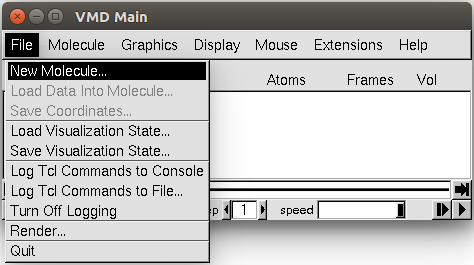
\includegraphics[scale=0.5]{vmd1}
\par\end{centering}
\caption{Snapshot of the main white box of VMD.}

\label{fig:vmd1}
\end{figure}

\begin{figure}
\begin{centering}
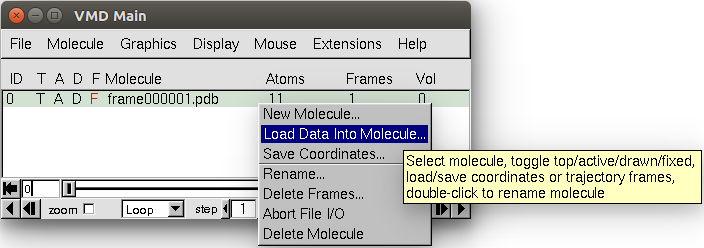
\includegraphics[scale=0.5]{vmd2}
\par\end{centering}
\caption{Snapshot of the \textquotedbl{}Load Coordinates into Molecule\textquotedbl{}
selection in VMD.}

\label{fig:vmd2}
\end{figure}


\newpage{}

 \bibliographystyle{elsarticle-num}
\bibliography{bibliography}

\newpage{} 
\end{document}
